\documentclass[11pt,a4paper,oldfontcommands]{memoir}
\usepackage[utf8]{inputenc}
% \usepackage[english]{babel}
\usepackage[T1]{fontenc}
\usepackage{microtype}
\usepackage[dvips]{graphicx}
\usepackage{xcolor}
\usepackage{times}
\usepackage{url}
\usepackage{comment}
\usepackage{amsmath}
\usepackage{tcolorbox}
\usepackage{float}
% \usepackage[<options>]{natbib}
% \renewcommand{\baselinestretch}{4.5}

%Includes "References" in the table of contents
% \usepackage[nottoc]{tocbibind}

\usepackage[
breaklinks=true,colorlinks=true,
linkcolor=blue,urlcolor=blue,citecolor=blue,% PDF VIEW
% linkcolor=black,urlcolor=black,citecolor=black,% PRINT
bookmarks=true,bookmarksopenlevel=2]{hyperref}

\usepackage{geometry}
% PDF VIEW
% \geometry{total={210mm,297mm},
% left=25mm,right=25mm,%
% bindingoffset=0mm, top=25mm,bottom=25mm}
% PRINT
\geometry{total={210mm,297mm},
left=20mm,right=20mm,
bindingoffset=10mm, top=25mm,bottom=25mm}

% \OnehalfSpacing
% \DoubleSpacing/
\linespread{1.3}

%%% CHAPTER'S STYLE
% \chapterstyle{bianchi}
% \chapterstyle{ger}
% \chapterstyle{madsen}
\chapterstyle{ell}
%%% STYLE OF SECTIONS, SUBSECTIONS, AND SUBSUBSECTIONS
% \setsecheadstyle{\Large\bfseries\sffamily\raggedright}
% \setsubsecheadstyle{\large\bfseries\sffamily\raggedright}
% \setsubsubsecheadstyle{\bfseries\sffamily\raggedright}


%%% STYLE OF PAGES NUMBERING
\pagestyle{companion}\nouppercaseheads 
\pagestyle{headings}
\pagestyle{Ruled}
\pagestyle{plain}
\makepagestyle{plain}
\makeevenfoot{plain}{\thepage}{}{}
\makeoddfoot{plain}{}{}{\thepage}
\makeevenhead{plain}{}{}{}
\makeoddhead{plain}{}{}{}


\maxsecnumdepth{subsection} % chapters, sections, and subsections are numbered
\maxtocdepth{subsection} % chapters, sections, and subsections are in the Table of Contents

% 
% \usepackage[dou­blespac­ing]{setspace}

%%%---%%%---%%%---%%%---%%%---%%%---%%%---%%%---%%%---%%%---%%%---%%%---%%%

\begin{document}

%%%---%%%---%%%---%%%---%%%---%%%---%%%---%%%---%%%---%%%---%%%---%%%---%%%
%   TITLEPAGE
%
%   due to variety of titlepage schemes it is probably better to make titlepage manually
%
%%%---%%%---%%%---%%%---%%%---%%%---%%%---%%%---%%%---%%%---%%%---%%%---%%%
\thispagestyle{empty}

{%%%
\sffamily
\centering
\Large

~\vspace{\fill}

{\huge 
A Code inspection tool for debugging Autumn's Context-Sensitive Grammars
}

\vspace{2.5cm}

{\LARGE
Gerard Nicolas
}

\vspace{3.5cm}

A thesis submitted in partial fulfillment for the\\
degree of Master in Computer Sciences\\[1em]
in the\\[1em]
Faculty EPL\\
University UCL

\vspace{3.5cm}

Supervisors: \\Prof. Kim Mens, \\Phd. student Nicolas Laurent

\vspace{\fill}

August 2017

%%%
}%%%

\cleardoublepage
%%%---%%%---%%%---%%%---%%%---%%%---%%%---%%%---%%%---%%%---%%%---%%%---%%%
%%%---%%%---%%%---%%%---%%%---%%%---%%%---%%%---%%%---%%%---%%%---%%%---%%%

\begin{abstract}
The debuging process is a crutial part of the lifetime of any projects. Unfortunately general purpose debuggers cannot provide the level of abstraction needed to reason efficiently on grammar developpement related errors.

We introduce a debugging tool to Autumn context-sensitive grammar. The goal is to provide the developpers with a tool that expose high level abstractions that represents the structure he reason about more closely, allowing him to track errors and resolve them more easily.
\end{abstract}

\cleardoublepage

\renewcommand{\abstractname}{Acknowledgements}
\begin{abstract}
I would like to thank my mentor Kim Mens and PHD student Nicolas Laurent for their support and understanding.
\end{abstract}

\cleardoublepage

\tableofcontents

\clearpage


%%%---%%%---%%%---%%%---%%%---%%%---%%%---%%%---%%%---%%%---%%%---%%%---%%%
%%%---%%%---%%%---%%%---%%%---%%%---%%%---%%%---%%%---%%%---%%%---%%%---%%%

%%%---%%%---%%%---%%%---%%%---%%%---%%%---%%%---%%%---%%%---%%%---%%%---%%%
\chapter{Introduction and motivation}

%%%---%%%---%%%---%%%---%%%---%%%---%%%---%%%---%%%---%%%---%%%---%%%---%%%

	\begin{itemize}
		\item debugger for autumn
		\item not a debugger a proprement parler
		\item it actually is more like a code anylizer but for the rest of this paper we will refer to it as a ``debugging tool''
		\item autumn is a parser library
		\item what is special about autumn ?
		\item Ok autumn is cool, but have no debugger
		\item debugger are important why ?
		\item ok lets read about it
	\end{itemize}

	\begin{itemize}
		\item language tools = pretty cool
		\item programmers are building domain-specific languages
		\item many mainstream programming and markup language possess context-sensitive features. 
		\item however few solution exists for true context-sensitive parsing
		\item Autumn is a context sensitive parser combinator developped in Kotlin.
		\item particularity : it can deal with context sensitive grammars.
		\item debuggers = important tool = expose the underlying execution and helps detect issues and correct them
		\item traditional debuggers =  generic mechanisms to explore and exhibit the execution stack and system state
		\item grammar developpement and parsing developper = domain-specific reasoning
		\item creates gap between the debugging needs and the debugging support.
		\item Writting and debugging grammar is tricky business. 
		\item Errors throwed while executing grammar are rarely useful for debuging.
		\item we don't know if the error comes from the grammar or the input.
		\item we propose a code inspection tool to help expose those higher level concepts 
		\item code inspection tool and intellij IDE plugin designed to work with Autumn Grammars.
		\item provide the user with relevant information he can easily reason with to track and identify potential issues in a much easier way.
		\item to convince ourselves, lets have a look at an example. (example showing unhelpful error message and highlighting what kind of information would be more relevant)
	\end{itemize}

		The goal is to simplify the life of the developper when writting grammars.
	Just as developers use IDEs (integrated development environments) to dramatically improve their productivity, programmers need a sophisticated development environment for building, understanding, and debugging grammars. 

	\begin{comment}

		Current grammar formalisms struggle to express context-sensitive features. Most solutions lack context transparency: they make grammars hard to write, maintain and compose by hardwiring context through the entire grammar. Instead, we approach context-sensitive parsing through the idea that parsers may recall previously matched input (or data derived therefrom) in order to make parsing decisions. We make use of mutable parse state to enable this form of recall.

		Writting and debugging grammar is tricky business. Errors throwed while executing grammar are rarely useful for debuging. The log doesnt tell us if the error comes from the grammar or the input. The dump file is really not managable. So the approach is to simply the life of the use by writting a debugger. 

		Debuggers are comprehension tools. They are often used by developers to under- stand the run-time behavior of software and elicit run-time information [18,19]. In test-driven development the debugger is used as a development tool given that it provides direct access to the running system [20]. Despite their importance, most debuggers only provide low-level operations that do not capture user intent and standard user interfaces that only display generic information. These issues can be addressed if developers are able to create domain-specific debuggers adapted to their problems and domains. Domain- specific debuggers can provide features at a higher level of abstraction that (i) match the domain model of software applications and (ii) group contextual information from various sources.

		In this section we establish and motivate four requirements that an infrastruc- ture for developing domain-specific debuggers should support, namely: domain- specific user interfaces, domain-specific debugging operations, automatic discov- ery and dynamic switching\cite{moldable}.


	\end{comment}
%%%---%%%---%%%---%%%---%%%---%%%---%%%---%%%---%%%---%%%---%%%---%%%---%%%---%%%---%%%---%%%---%%%---%%%---%%%---%%%---%%%---%%%---%%%---%%%---%%%

%%%---%%%---%%%---%%%---%%%---%%%---%%%---%%%---%%%---%%%---%%%---%%%---%%%---%%%---%%%---%%%---%%%---%%%---%%%---%%%---%%%---%%%---%%%---%%%---%%%	



	 %The Dump file is really not managable. 

%%%---%%%---%%%---%%%---%%%---%%%---%%%---%%%---%%%---%%%---%%%---%%%---%%%
% \part{Research}
%%%---%%%---%%%---%%%---%%%---%%%---%%%---%%%---%%%---%%%---%%%---%%%---%%%


%%%%----%%%%----%%%%----%%%%----%%%%----%%%%----%%%%----%%%%----%%%%----%%%%----%%%%----%%%%----%%%%----%%%%----%%%%----%%%%----%%%%----%%%%----%%%%----%%%%----
\chapter{Based Material}
%%%%----%
		%%%%----%%%%----%%%%----%%%%----%%%%----%%%%----%%%%----%%%%----%%%%----%%%%----%%%%----%%%%----%%%%----%%%%----%%%%----%%%%----%%%%----%%%%----%%%%----
		%
%%%%----%%%%----%%%%----%%%%----%%%%----%%%%----%%%%----%%%%----%%%%----%%%%----%%%%----%%%%----%%%%----%%%%----%%%%----%%%%----%%%%----%%%%----%%%%----%%%%----
	\section{Parsing expression grammar} 
	%%%%----%%%%----%%%%----%%%%----%%%%----%%%%----%%%%----%%%%----%%%%----%%%%----%%%%----%%%%----%%%%----%%%%----%%%%----%%%%----%%%%----%%%%----%%%%----%%%%----
	%
	%
%%%%----%%%%----%%%%----%%%%----%%%%----%%%%----%%%%----%%%%----%%%%----%%%%----%%%%----%%%%----%%%%----%%%%----%%%%----%%%%----%%%%----%%%%----%%%%----%%%%----

\begin{itemize}
	\item PEG = type of analytic formal grammar closely related to the family of top-down parsing languages
	\item similar to context-free grammars (CFGs) but PEGs cannot be ambiguous; if a string parses, it has exactly one valid parse tree.
	\item Formally, a parsing expression grammar consists of: A finite set N of nonterminal symbols. A finite set $\sum$ of terminal symbols that is disjoint from N. A finite set P of parsing rules. An expression eS termed the starting expression.
	\item Each parsing rule in P has the form A $<-$ e, where A is a nonterminal symbol and e is a parsing expression. A parsing expression is a hierarchical expression similar to a regular expression, which is constructed in the following fashion:  
	\begin{itemize}
		\item An atomic parsing expression consists of: any terminal symbol, any nonterminal symbol, or the empty string.
		\item Given any existing parsing expressions e, e1, and e2, a new parsing expression can be constructed using the following operators: Sequence Ordered choice Zero-or-more One-or-more Optional And-predicate Not-predicate
	\end{itemize}
	\item desirable properties: closure under composition, built-in disambiguation, unifica- tion of syntactic and lexical concerns, and closely matching programmer intuition.
	\item struggle with left-recursive grammar rules : infinite recursion
	\item  These include parser generators (like the venerable Yacc) and more recently parser combinator libraries [5].
\end{itemize}

\begin{comment}
	\item Most of the work on parsing has been built on top of Chomsky’s context-free grammars (CFGs). 
	\item Ford’s parsing expression grammars (PEGs) [3] are an alternative formal- ism exhibiting interesting properties. Whereas CFGs use non-deterministic choice between alternative constructs, PEGs use prioritized choice. This makes PEGs unambiguous by construction.
	\item CFGs are generative: they describe a language, and the grammar itself can be used to enumerate the set of sen- tences belonging to that language. PEGs on the other hand are recognition-based: they describe a predicate indicating whether a sentence belongs to a language.
	\item The recognition-based approach is a boon for program- mers who have to find mistakes in a grammar. It also en- ables us to add new parsing operators, as we will see in sec- tion 4. These benefits are due to two PEG characteristics. (1) The parser implementing a PEG is generally close to the grammar, making reasoning about the parser’s operations easier. This characteristic is shared with recursive-descent CFG parsers. (2)
	\item The single parse rule: attempting to match a parsing expression (i.e. a sub-PEG) at a given input posi- tion will always yield the same result (success or failure) and consume the same amount of input. This is not the case for CFGs. For example, with a PEG, the expression (a*) will al- ways greedily consume all the a’s available, whereas a CFG could consume any number of them, depending on the gram- mar symbols that follow.
	\item First is the problem of left-recursion, an issue which PEGs share with recursive- descent CFG parsers. This is sometimes singled out as a rea- son why PEGs are frustrating to use [11].
	\item Solutions that do support left-recursion do not always let the user choose the associativity of the parse tree for rules that are both left- and right-recursive; either because of technical limitations [1] or by conscious design [10]. We contend that users should be able to freely choose the associativity they desire.
	\item Whitespace handling is another problem. Traditionally, PEG parsers do away with the distinction between lexing and parsing. This alleviates some issues with traditional lexing: different parts of the input can now use different lex- ing schemes, and structure is possible at the lexical level (e.g. nested comments) [3].
	\item However, it means that whites- pace handling might now pollute the grammar as well as the generated syntax tree. Finally, while PEGs make linear- time parsing possible with full memoization1, there is a fine balance to be struck between backtracking and memoiza- tion [2]. Memoization can bring about runtime speedups at the cost of memory use. Sometimes however, the run time overhead of memoization nullifies any gains it might bring.
	\item  Error reporting tends to be poor, and is not able to ex- ploit knowledge held by users about the structure of their grammars. Syntax trees often consist of either a full parse tree that closely follows the structure of the grammar, or data structures built on the fly by user-supplied code (seman- tic actions). Both approaches are flawed: a full parse tree is too noisy as it captures syntactic elements with no seman- tic meaning, while tangling grammatical constructs and se- mantic actions (i.e. code) produces bloated and hard-to-read grammars. Generating trees from declarative grammar anno- tations is possible, but infrequent.
	\item recognition-based formal foundation for describing machine- oriented syntax
	\item Where CFGs express nondeter- ministic choice between alternatives, PEGs instead use prioritized choice
	\item A linear-time parser can be built for any PEG, avoiding both the com- plexity and fickleness of LR parsers and the inefficiency of gener- alized CFG parsing. While PEGs provide a rich set of operators for constructing grammars, they are reducible to two minimal recogni- tion schemas developed around 1970, TS/TDPL and gTS/GTDPL, which are here proven equivalent in effective recognition power.
	\item Most language syntax theory and practice is based on generative systems, such as regular expressions and context-free grammars, in which a language is defined formally by a set of rules applied re- cursively to generate strings of the language. A recognition-based system, in contrast, defines a language in terms of rules or predi- cates that decide whether or not a given string is in the language.
	\item Simple languages can be expressed easily in either paradigm. For example, ${s ∈ a\* | s = (aa)^n}$ is a generative definition of a trivial language over a unary character set, whose strings are “constructed” by concatenating pairs of a’s. In contrast, ${s ∈ a\* | (|s| mod 2 = 0)}$ is a recognition-based definition of the same language, in which a string of a’s is “accepted” if its length is even.
	\item Chomsky’s generative system of grammars, from which the ubiqui- tous context-free grammars (CFGs) and regular expressions (REs) arise, was originally designed as a formal tool for modelling and analyzing natural (human) languages. Due to their elegance and expressive power, computer scientists adopted generative grammars for describing machine-oriented languages as well. The ability of a CFG to express ambiguous syntax is an important and powerful tool for natural languages. Unfortunately, this power gets in the way when we use CFGs for machine-oriented languages that are intended to be precise and unambiguous. Ambiguity in CFGs is difficult to avoid even when we want to, and it makes general CFG parsing an inherently super-linear-time problem [14, 23].
	\item A PEG may be viewed as a formal description of a top-down parser. Two closely related prior systems upon which this work is based were developed primarily for the purpose of studying top-down parsers [4, 5].
	\item PEGs have far more syntactic expressiveness than the LL(k) language class typically associated with top-down parsers, however, and can express all deterministic LR(k) languages and many others, including some non-context-free languages. Despite their considerable expressive power, all PEGs can be parsed in lin- ear time using a tabular or memoizing parser [8].
	\item he recognition-oriented nature of PEGs creates a natural affinity in terms of syntactic expressiveness and parsing efficiency.
\end{comment}

The fundamental difference between context-free grammars and parsing expression grammars is that the PEG's choice operator is ordered.

\begin{itemize}
	\item DSLs are generally very high-level languages tailored to specific tasks.
	\item DSLs are particularly important to software development because they represent a more natural, high-fidelity, robust, and maintainable means of encoding a problem than simply writing software in a general- purpose language.
\end{itemize}


\paragraph{Parsing} Imagine a maze with a single entrance and single exit that has words written on the floor. Every path from entrance to exit generates a sentence by “saying” the words in sequence. In a sense, the maze is analogous to a grammar that defines a language.

You can also think of a maze as a sentence recognizer. Given a sentence, you can match its words in sequence with the words along the floor. Any sentence that successfully guides you to the exit is a valid sentence in the language defined by the maze. 

At almost every word, the recog- nizer must make a decision about the interpretation of a phrase or subphrase. Sometimes these decisions are very complicated. For example, some decisions require information about previous decision choices or even future choices. Most of the time, however, decisions need just a little bit of lookahead information.

\paragraph{Grammar} To understand grammars and to understand their capabilities and limitations, you need to learn about the nature of computer languages.

Represent grammar as a state machine; states and transitions labeled with vocabulary symbols. The transitions are directed connections that govern navigation among the states. Machine execution begins in state s0, the start state, and stops in s4, the accept state.

The machine can also generate invalid sentences, such as “Your truck is sad and sad.” Grammatical does not imply sensible. For example, “Dogs revert vacuum bags” is grammatically OK but doesn’t make any sense. 
The difference between the regular and context-free languages is the differ- ence between a state machine and the more sophisticated machines in the next section. The essential weakness of a state machine is that it has no memory of what it generated in the past. 
Trees Such trees are called derivation trees when generating sentences and parse trees when recognizing sen- tences.
It turns out that the humble stack is the perfect memory structure to solve both word dependency and order problems.4 Adding a stack to a state machine turns it into a pushdown machine. A state machine is analogous to a stream of instructions trapped within a single method, unable to make method calls. A pushdown machine, on the other hand, is free to invoke other parts of the machine and return just like a method call. The stack allows you to partition a machine into submachines. These submachines map directly to the rules in a grammar.

\paragraph{Ambiguousity}


As we all know, English and other natural languages can be delight- fully ambiguous. Any language with an ambiguous sentence is consid- ered ambiguous, and any sentence with more than a single meaning is ambiguous. Sentences are ambiguous if at least one of its phrases is ambiguous. Here is an ambiguous faux newspaper headline: “Bush appeals to democrats.” In this case, the verb appeals has two mean- ings: “is attractive to” and “requests help from.” This is analogous to operator overloading in computer languages, which makes programs hard to understand just like overloaded words do in English.

For example, a syntax diagram for C can generate statement i*j; following the path for both a multiplicative expression and a variable definition (in other words, j is a pointer to type i). To learn more about the relationship of ambiguous languages to ANTLR grammars,

Complex language generation enforces word dependencies and order requirements. Your brain enforces these constraints by subconsciously creating a tree structure. It does not generate sentences by thinking about the first word, the second word, and so on, like a simple state machine. It starts with the overall sentence concept, the root of the tree structure. From there the brain creates phrases and subphrases until it reaches the leaves of the tree structure. From a computer scientist’s point of view, generating a sentence is a matter of performing a depth-first tree walk and “saying” the words represented by the leaves. The implicit tree structure conveys the meaning.
Sentence recognition occurs in reverse. Your eyes see a simple list of words, but your brain subconsciously conjures up the implicit tree structure used by the person who generated the sentence.

\section{difficulties}
there are two very common difficulties encountered by grammar developers: Understanding why a grammar fragment results in a parser nondeterminism and determining why a generated parser incorrectly interprets an input sentence.

%%%---%%%---%%%---%%%---%%%---%%%---%%%---%%%---%%%---%%%---%%%---%%%---%%%---%%%---%%%---%%%---%%%---%%%---%%%---%%%---%%%---%%%---%%%---%%%---%%%
\section{Autumn Parsing Library}
%%%---%%%---%%%---%%%---%%%---%%%---%%%---%%%---%%%---%%%---%%%---%%%---%%%---%%%---%%%---%%%---%%%---%%%---%%%---%%%---%%%---%%%---%%%---%%%---%%%

	Autumn is a context sensistive parsing library.
	\begin{itemize}
		\item Autumn is different from other parsing lib because it deals with true context sensitivity.
		\item context-sensitive in parsing = tricky (context transparency) however lots of mainstream languages exhibit context sensitive features.
		\item most grammar formalism lack context transparency, they handle context sensitivity with ad-hoc code outside of the scope of parsing theory.
		\item  custom memoization and error han- dling strategies.

	\end{itemize}

%%%---%%%---%%%---%%%---%%%---%%%---%%%---%%%---%%%---%%%---%%%---%%%---%%%---%%%---%%%---%%%---%%%---%%%---%%%---%%%---%%%---%%%---%%%---%%%---%%%
	\subsection{Context sensitivity}
%%%---%%%---%%%---%%%---%%%---%%%---%%%---%%%---%%%---%%%---%%%---%%%---%%%---%%%---%%%---%%%---%%%---%%%---%%%---%%%---%%%---%%%---%%%---%%%---%%%

	\begin{itemize}
		\item grammar needs to remember what was previously matched to make a decision
		\item Autumn uses a parse wide state to remember context
		\item problem with stateful parsing : context transparency : Sometimes parse has to backtrack (explain here what backtracking is) and therefore need to undo changes made to the state.
		\item One might think that it can be easily done with a simple construct that undo the change on failure
		\item tricky part is : some parsers might be success full but because one of its ancestor failed, its changes has to be reverted anyway.
		\item Autumn's approach to deal with context transparancy : principled stateful parsing
		\item Principled stateful parsing define a set of primitive state manipulation operations that allows us to get an image of the parse state at a specific time and allow us to revert the state to that of the image. (consequence : we can backtrack safely)
	\end{itemize}

	A grammatical construct is context-transparent if it is unaware of the context shared between its ancestors and its descendants.
	
	Stateful parsing is not enough to deal with context sensitivity as it is not context-transparent. (We need to make sure that parsers combinator doesnt backtrack)

	% Stateful parsers also are not context-transparent, as they must ensure that no unforeseen backtracking or memoization takes place. For instance, if a parser a manipulates the state and its callers do not expect it to backtrack, it cannot be swapped for a parser c(a) (where c is some parser combinator) without first ensuring that c(a) never backtracks over a.

	% As the previous section has shown, enabling the definition of context-sensitive languages without jeopardizing maintainability, composability or even safety is no easy feat. We put forward the notion of context transparency as the gold standard that a context sensitive parsing mechanism needs to meet in order to be considered sufficiently practical.
	% Data-dependent grammars, monadic parsers, DCGs and attribute grammars are not context-transparent because of the need to explicitly pass values around. For instance, consider two data-dependent grammars4: a grammar for a Python- like language with significant indentation, in which the rules for block-level constructs (statements, definitions) are paremeterized by the indentation level; and a grammar for a generic macro definition language (e.g., GNU M4). We want to compose these two languages such that macro definitions may appear anywhere where definitions can appear in our Python-like language. Additionally, we want macro bodies to include Python-like code.
	% The issue is that the rules in the macro language grammar know nothing about indentation level, yet the indentation level needs to be shared between the block holding the macro definition and the Python-like code appearing inside macro definitions. In this case, the lack of context transparency would force us to rewrite all rules in the macro language grammar to carry around the indentation level.
	% Stateful parsers also are not context-transparent, as they must ensure that no unforeseen backtracking or memoization takes place. For instance, if a parser a manipulates the state and its callers do not expect it to backtrack, it cannot be swapped for a parser c(a) (where c is some parser combinator) without first ensuring that c(a) never backtracks over a.
	% Lack of context-transparency makes grammars hard to reason about, hence hard to write and to maintain: refactoring, extending or composing grammars becomes particularly challenging, because each change to a rule might entail the need to modify all rules through which it is (transitively) reachable. In stateful parsers, such changes are liable to introduce undesired backtracking or memoization.
	% We suggest a simple solution: use stateful parsing (which does not thread context through the grammar), but undo state changes upon backtracking and allow the memoization of state changes. And to achieve this, we introduce a new context sensitivity handling discipline: principled stateful parsing.

%%%---%%%---%%%---%%%---%%%---%%%---%%%---%%%---%%%---%%%---%%%---%%%---%%%---%%%---%%%---%%%---%%%---%%%---%%%---%%%---%%%---%%%---%%%---%%%---%%%
	\subsection{Principled Stateful Parsing}
%%%---%%%---%%%---%%%---%%%---%%%---%%%---%%%---%%%---%%%---%%%---%%%---%%%---%%%---%%%---%%%---%%%---%%%---%%%---%%%---%%%---%%%---%%%---%%%---%%%


% If the execution of a parser were linear, simply read- ing/writing to this state would suffice. Unfortunately, parsers must sometimes perform speculative executions that may fail further down the line, a phenomenon called backtracking. When backtracking occurs, all state changes in the specu- lative execution being backtracked over must be reversed. Hence, we need an operation that can take a snapshot of the state at a given point, and an operation that can restore the state described by such a snapshot.

	\subsubsection{Parse State}
	\begin{itemize}
		\item state = passing context around implicitly
		\item if execution = linear, reading/writting to this state would suffice.
		\item althought because of backtracking (speculative execution) : we need to reverse the state.
	\end{itemize}
	\subsubsection{Parsers} A parser represents a computation over the parse state that either succeeds or fails and has side effects on the parse state.
	\subsubsection{Primitive Operations}
	To deal with backtracking we need operations that can take a picture of the state at a particular time and restore it. 4 operations are used to manipulate states:
	\begin{itemize}
		\item snapshot : capture of the state at a specific point during the execution. 
		\item restore : The restore operation takes a snapshot as input and returns a transformation that brings the state to that described by the snapshot.
		\item diff : The diff operation returns a DELTA object representing the difference between a snapshot and the current state
		\item merge : The merge operation takes a delta as input and returns a transformation that appends this delta to the input state.
	\end{itemize}


		% \paragraph{context sensitivity} to express context-sensitive features: storing the matched input (or data derived thereof) in a mutable data store: the parse state.
		% \paragraph{Using State} to pass context around implicitly (context transparency).
		% \paragraph{Backtracking} can occur so we need to be able to reverse the state. This is done through a set of primitive operations that deals directly with the state.
		% \paragraph{State store} is in fact a log of operations applied.

		% % we established the relevance of context-sensitive parsing and introduced the notion of recall as a way to express context-sensitive features in terms of backreferences to previously matched input. We enable recall by storing the matched input (or data derived thereof) in a mutable data store: the parse state. This section expounds how principled stateful parsing is able to work with parse state while avoiding the usual pitfalls of stateful parsing (cf. sections 2.5 and 3).

		% % The point of using state is to pass context around implicitly, without the need to hardwire context in the grammar, hence achieving context transparency (cf. Section 3). If the execution of a parser were linear, simply reading/writing to this state would suffice. Unfortunately, parsers must sometimes perform speculative executions that may fail further down the line, a phenomenon called backtracking. When backtracking occurs, all state changes in the specu- lative execution being backtracked over must be reversed. Hence, we need an operation that can take a snapshot of the state at a given point, and an operation that can restore the state described by such a snapshot.
		% % Given these requirements, it helps to think of the parse state as a log of the operations applied to the state, which can be snapshot and rolled back as required. Appropriately, this is also how we formalize the parse state.
		% % Additionally, it is sometimes desirable to save the result of a speculative execution (whether it failed or not), i.e., the state changes it induced: a delta acquired by performing a diff between the states before and after the execution. It is also necessary to be able to merge these changes back into the state. The most straightforward application of the diff and merge capabilities is the memoization of parse results. However, other valuable use cases exist, such as longest- match parsing and left-recursive parsing (see Section 5.4).
		% % This motivates the need for four primitive state-manipulation operations: snapshot, restore, diff and merge. These opera- tions are described in section 4.2.3.

		% \subsubsection{example}
		% 	\paragraph{Significant whitespace}

%%%---%%%---%%%---%%%---%%%---%%%---%%%---%%%---%%%---%%%---%%%---%%%---%%%---%%%---%%%---%%%---%%%---%%%---%%%---%%%---%%%---%%%---%%%---%%%---%%%
	\section{Implementation}
%%%---%%%---%%%---%%%---%%%---%%%---%%%---%%%---%%%---%%%---%%%---%%%---%%%---%%%---%%%---%%%---%%%---%%%---%%%---%%%---%%%---%%%---%%%---%%%---%%%
	Explain how Autumn work from a high level ``intuitive'' level.

	Highlight the main classes and explain how they work together. Maybe a UML chart ?
%%%---%%%---%%%---%%%---%%%---%%%---%%%---%%%---%%%---%%%---%%%---%%%---%%%---%%%---%%%---%%%---%%%---%%%---%%%---%%%---%%%---%%%---%%%---%%%---%%%	
		\subsection{Important classes}
%%%---%%%---%%%---%%%---%%%---%%%---%%%---%%%---%%%---%%%---%%%---%%%---%%%---%%%---%%%---%%%---%%%---%%%---%%%---%%%---%%%---%%%---%%%---%%%---%%%

		\paragraph{Parsers} Parsers are function that return boolean, their implementation can be found in the parsers package and are implemented as extension functions of the grammar class
		\paragraph{Grammar} Main class: Explain how the main parsing algo works. And that every structures(maybe explain what are those structure and their purpose) are defined here.
		\paragraph{State/side effects/Undo structures} Explain how state is handled through undo structures, present the basic undo structures that are implemented and explain that the users can create custom structures for his needs.


	% \paragraph{Grammar} In practice, the grammar class works as the central node of the framework. It contains the state store, the input and contains the logic for applying side effects and reverting them.
	% \paragraph{Parsers} are defined as functions returning a boolean stating weither or not they succeeded. These functions can be combined to form more complex parsers called parser combinators. The package parsers include a serie of predifined primitive parsers ready for use.
	% \paragraph{Stateful parsing} Stack - undolist ... More can be implemented


% %%%---%%%---%%%---%%%---%%%---%%%---%%%---%%%---%%%---%%%---%%%---%%%---%%%---%%%---%%%---%%%---%%%---%%%---%%%---%%%---%%%---%%%---%%%---%%%---%%%
% %
% 	\section{Autumn grammar}
% %
% %%%---%%%---%%%---%%%---%%%---%%%---%%%---%%%---%%%---%%%---%%%---%%%---%%%---%%%---%%%---%%%---%%%---%%%---%%%---%%%---%%%---%%%---%%%---%%%---%%%
% Discuss briefly what it looks like syntactically speaking (Maybe not so interesting ?)

%%%---%%%---%%%---%%%---%%%---%%%---%%%---%%%---%%%---%%%---%%%---%%%---%%%
% \part{Contribution}
%%%---%%%---%%%---%%%---%%%---%%%---%%%---%%%---%%%---%%%---%%%---%%%---%%%


%%%---%%%---%%%---%%%---%%%---%%%---%%%---%%%---%%%---%%%---%%%---%%%---%%%---%%%---%%%---%%%---%%%---%%%---%%%---%%%---%%%---%%%---%%%---%%%---%%%
%
\chapter{Overview of the solution}
%
%%%---%%%---%%%---%%%---%%%---%%%---%%%---%%%---%%%---%%%---%%%---%%%---%%%---%%%---%%%---%%%---%%%---%%%---%%%---%%%---%%%---%%%---%%%---%%%---%%%
This chapter presents the main functionality of the debugging tool in all generalities and presents how it has been integrated with Intellij IDE as a GUI plugin.

\section{side note}

	\begin{itemize}
		\item at first : we wanted to work on top of the IDE debugger
		\item but from plugin it is difficult to access the implementation for the debugger
		\item made me think about what is important for debugging grammar ?
		\item important thing is to be able to see the execution trace of the parsers
		\item being able to look at the parse state the system was in when the parser was called
		\item to be able to see the portion of the input matched by the parser
		\item it is possible to access all this information without stopping the execution
		\item the syntax tree generated by the parse can by analyze and we can simulate time traveling in the parse execution
	\end{itemize}
% Discuss that having a debugger is one good thing, but as is, it is not very useful, we need a tool to harness its power. Explain that we build
% this plugin as a tool for the final user to use and develop his own parsers and grammar. This part has been created with the users need in mind
% to be as friendly user as possible.
	%%%---%%%---%%%---%%%---%%%---%%%---%%%---%%%---%%%---%%%---%%%---%%%---%%%---%%%---%%%---%%%---%%%---%%%---%%%---%%%---%%%---%%%---%%%---%%%---%%%
	\section{Overview of the fonctionality}

	%%%---%%%---%%%---%%%---%%%---%%%---%%%---%%%---%%%---%%%---%%%---%%%---%%%---%%%---%%%---%%%---%%%---%%%---%%%---%%%---%%%---%%%---%%%---%%%---%%%
	At this point we know the context, we know autumn and we know the motivations. From here we don't discuss why but how.

	\begin{itemize}
		\item Autumn implementation of parser as function -> changed into objects to create hooks for debugger.
		\item neet to rewrite java grammar to reflect changes in the parsers implementation
		\item debugger is a function that is hooked on the execution of each parsers
		\item during execution a syntax tree is build
		\item each node of the syntax tree contains informations about the parse state at the moment of the parser invocation
		\item those information can then be processed and displayed on a GUI for the developper to reason about
		\item ULM chart of the debugger and how it connects to autumn
	\end{itemize}



	% We developped a debugger, to do so we had to adapt autumn parsers. Parsers were initially boolean functions, we transformed them into objects that can be manipulated and stored to remember which parsers were called and in which order during runtime
	\begin{itemize}
		\item debuging tool = hook on top of parser's definition
		\item builds up a syntax tree
		\item which is then read and displayed by a GUI
		\item the GUI is implemented as a IDE plugin
	\end{itemize}

	\subsection{Intellij plugin}

	\begin{itemize}
		\item intellij plugin is essentially a panel that can be docked on top of the IDE
		\item it presents the data in several different forms
		\item the data can then be filtered to pinpoint specific problems
	\end{itemize}

	\begin{figure}[h]
		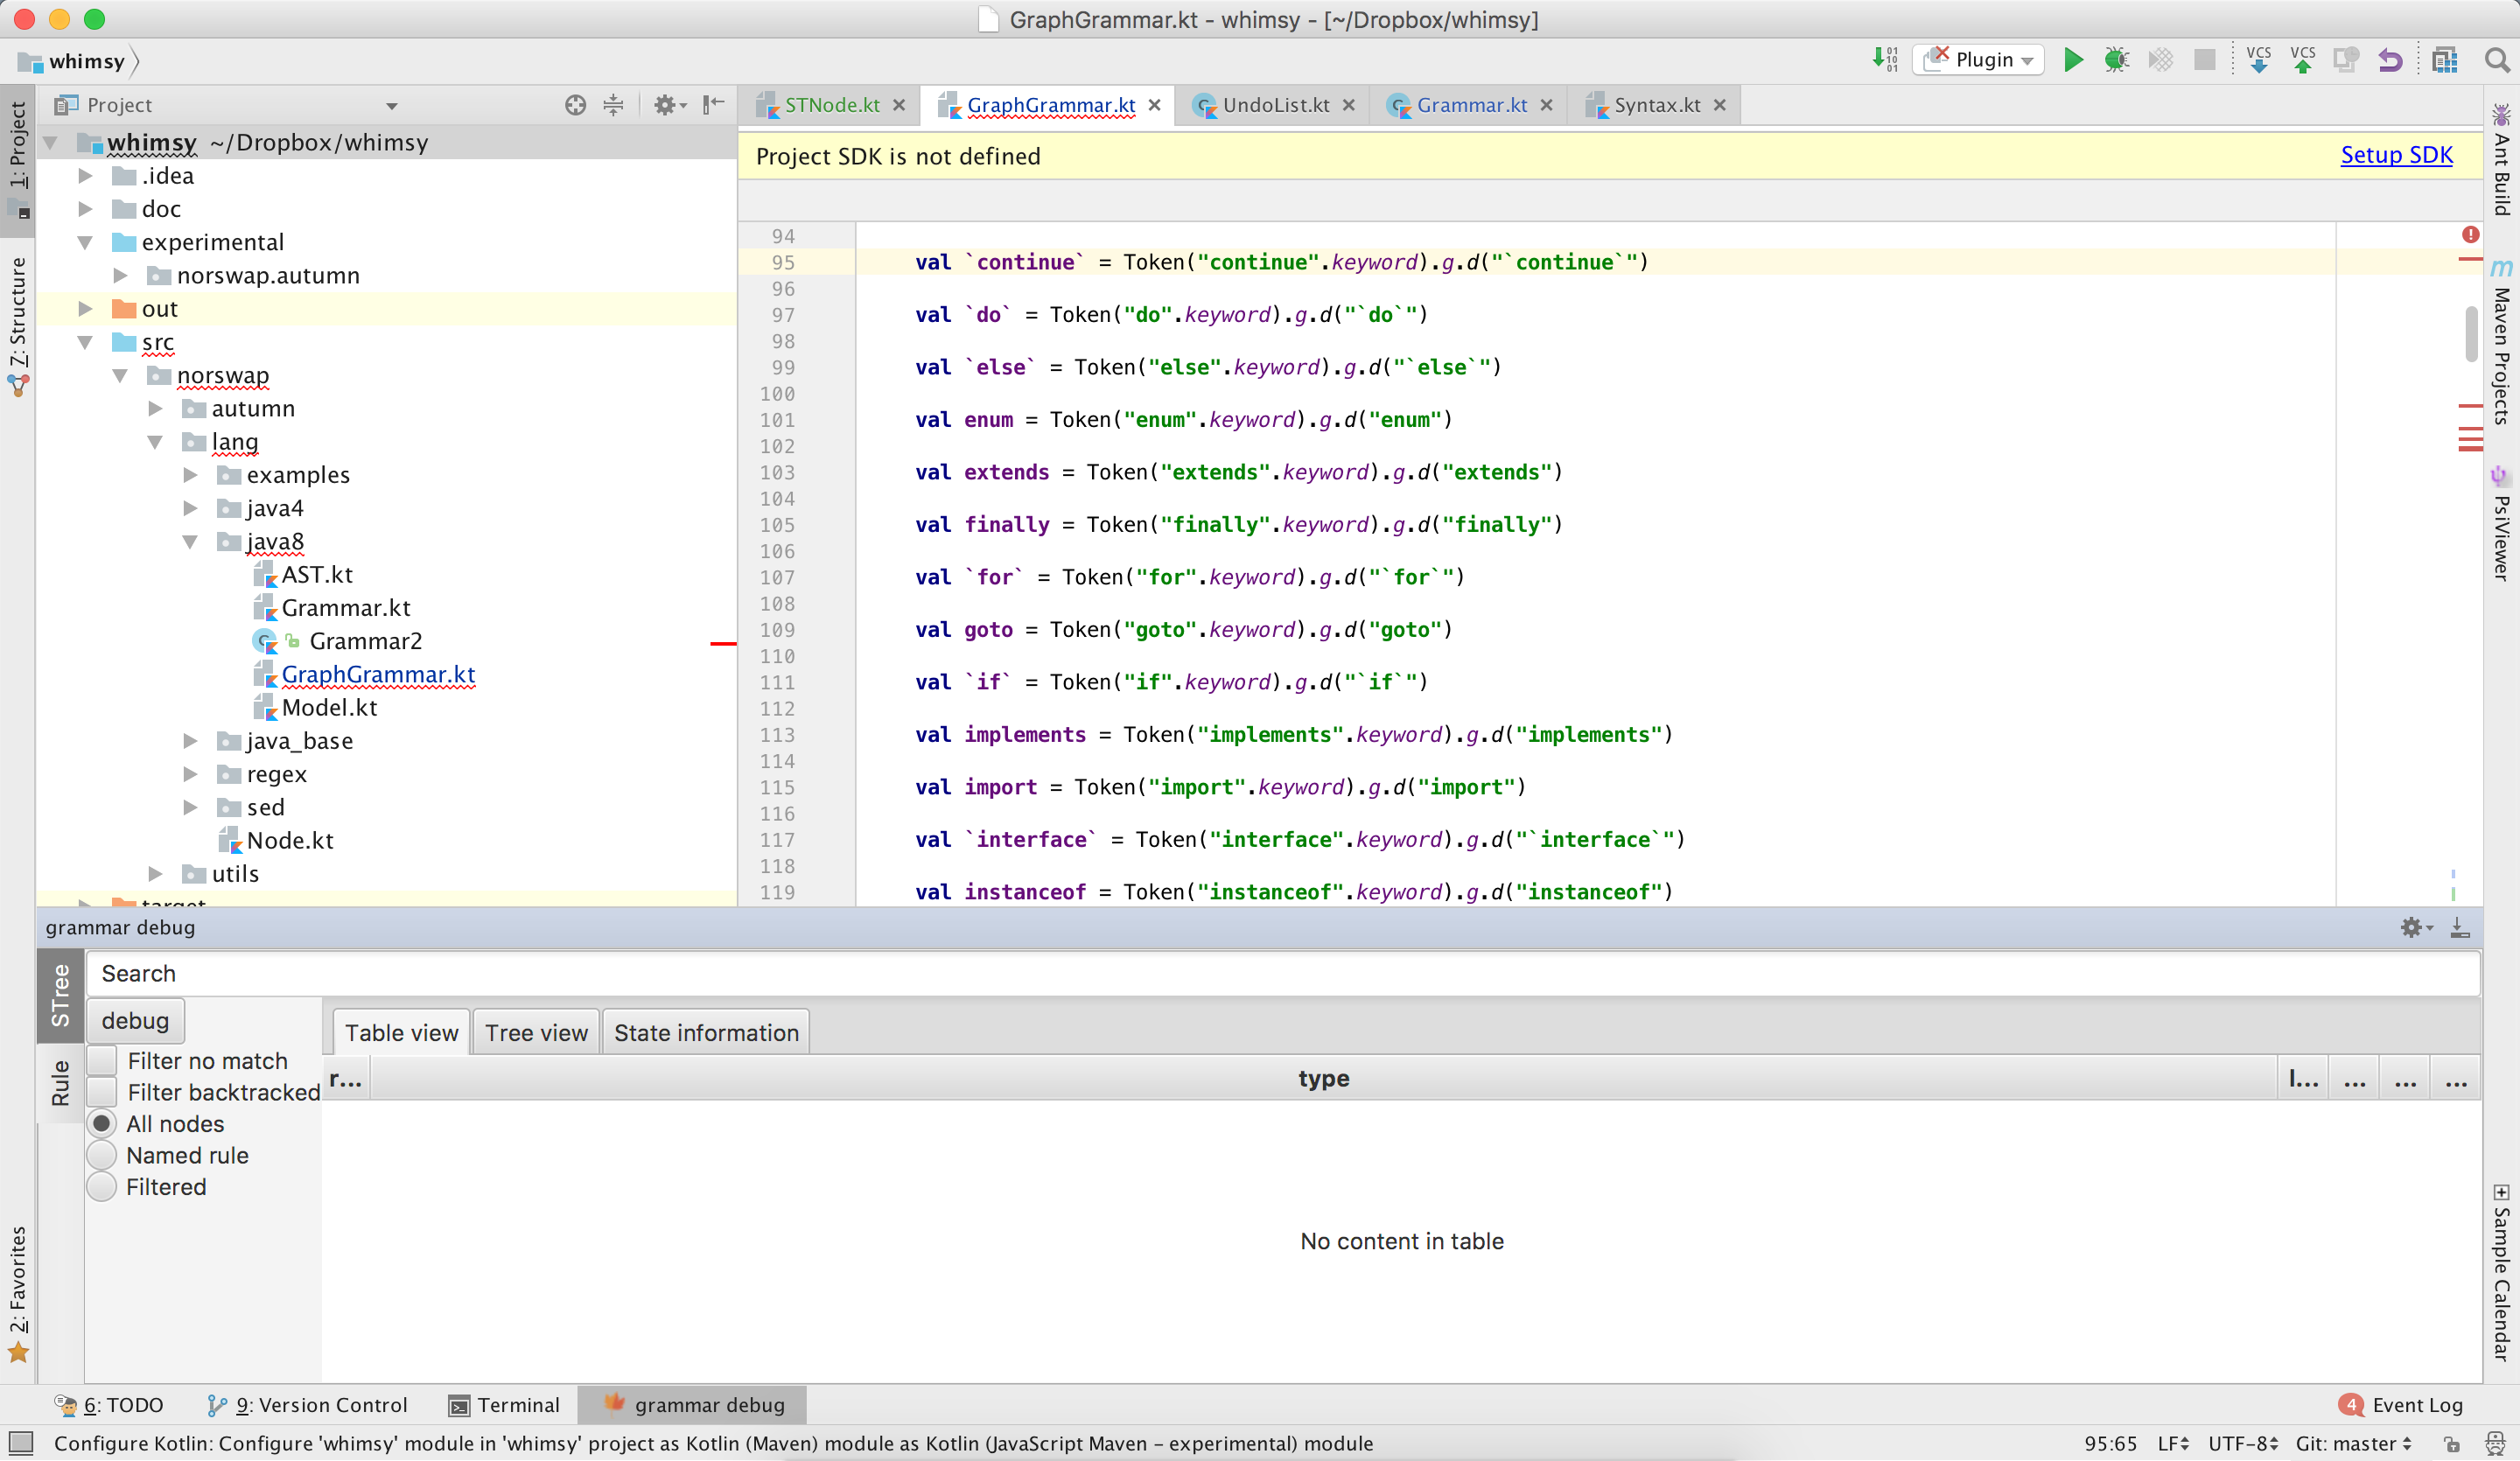
\includegraphics[width=1\textwidth] {ressources/intj_plug}
		\caption{IDE GUI for Autumn's debuggin tool} 
		\label{fig:intj_plug}
	\end{figure}

		% \paragraph{The debugger} works a posteriori, that means that it attempt to parser the file using the provided grammar and then display useful information about the parse. At first, the way we invision the debugger was more in the line of what general purpose debuggers do, executing the code and stopping at breakpoints, allowing the user to step into, over or resume the execution of the code. We wanted our debugger to work as a layer on top of Intellij's general purpose debugger. However, the difficulties of working with Intellij's debugger for the developpement of a plugin lead us to rething our solution.

		% We tried to get in the shoes of the grammar developper, while trying to troubleshoot his work, what does he really need to know ? The most important information for him is to be able to see which rule of the grammar has matched with what part of the input, and to be able to follow the sequence of parser calls. All those information are available almost for free. Throughout its execution, Autumn maintain a log of modification of the state, it is therefore possible to retrace the execution of the parsers using the syntax tree and regenerating the state corresponding to the call of a specific parser. So in practice, we eliminated the need to stop the execution at one point since we can display the execution trace and regenerate the state in which the parser was during the call, effectively providing the user with the tools needed to analyze the execution of the parser and similating the step in, over and backward a general purpose debugger would have.


		\begin{figure}[h]
			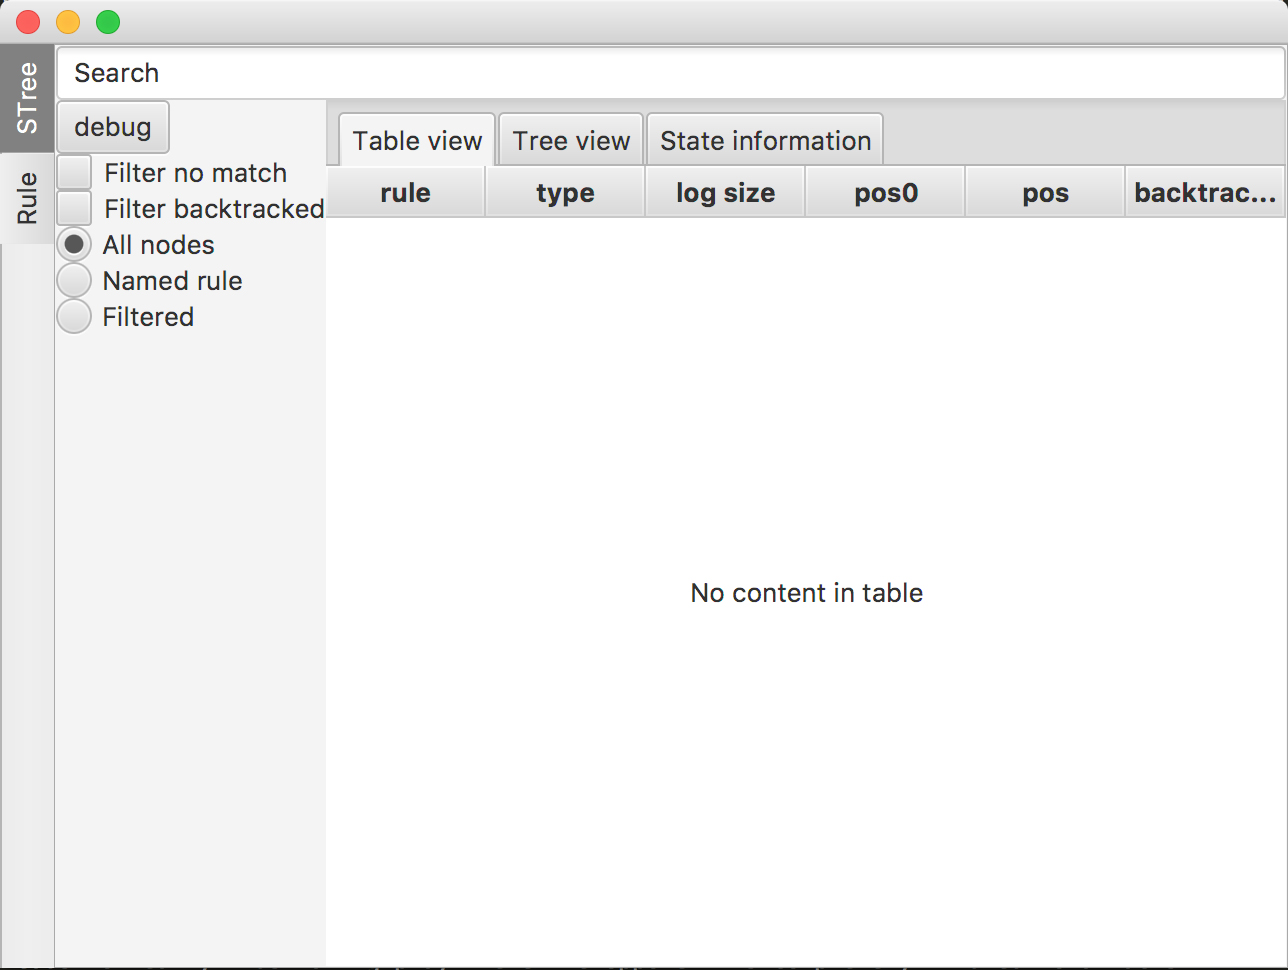
\includegraphics[width=1\textwidth] {ressources/stand_alone}
			\caption{Stand alone view - the debugger GUI can be executed independetly from the IDE albeit some restrictions} 
			\label{fig:stand_alone}
		\end{figure}


		\begin{figure}[h]
			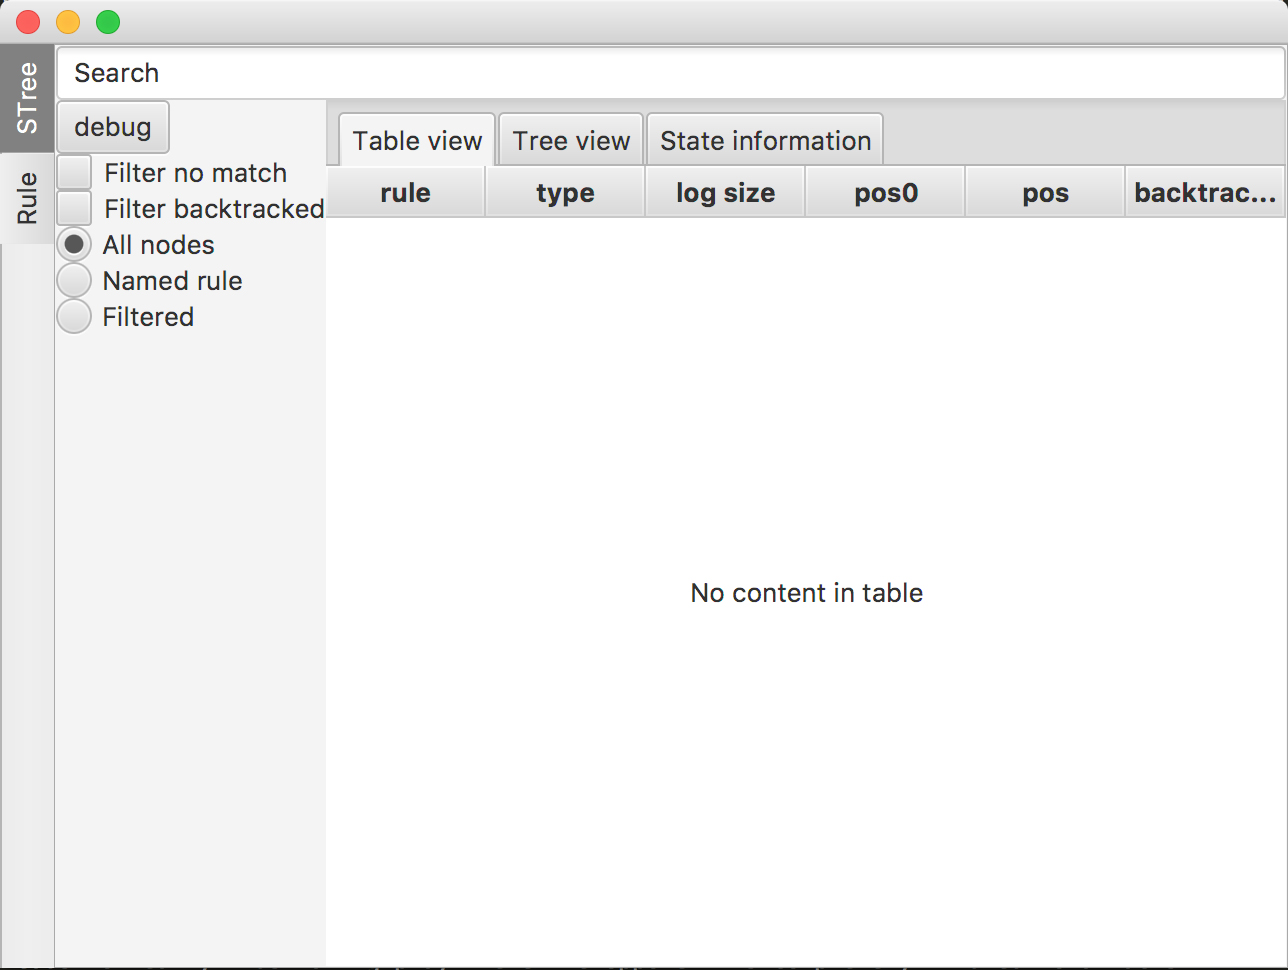
\includegraphics[width=1\textwidth] {ressources/stand_alone}
			% \caption{Stand alone view - the debugger GUI can be executed independetly from the IDE albeit some restrictions} 
			% \label{fig:stand_alone_detailed}
		\end{figure}


		%%%---%%%---%%%---%%%---%%%---%%%---%%%---%%%---%%%---%%%---%%%---%%%---%%%---%%%---%%%---%%%---%%%---%%%---%%%---%%%---%%%---%%%---%%%---%%%---%%%
		\subsection{Views}
		%%%---%%%---%%%---%%%---%%%---%%%---%%%---%%%---%%%---%%%---%%%---%%%---%%%---%%%---%%%---%%%---%%%---%%%---%%%---%%%---%%%---%%%---%%%---%%%---%%%
		\paragraph{Table view - Execution trace} The table view highlight the execution sequence of the parsers

		\begin{itemize}
			\item execution trace
			\item allow to see the sequence of parsers that were called chronologically
		\end{itemize}

		\begin{figure}[h]
			\centering
			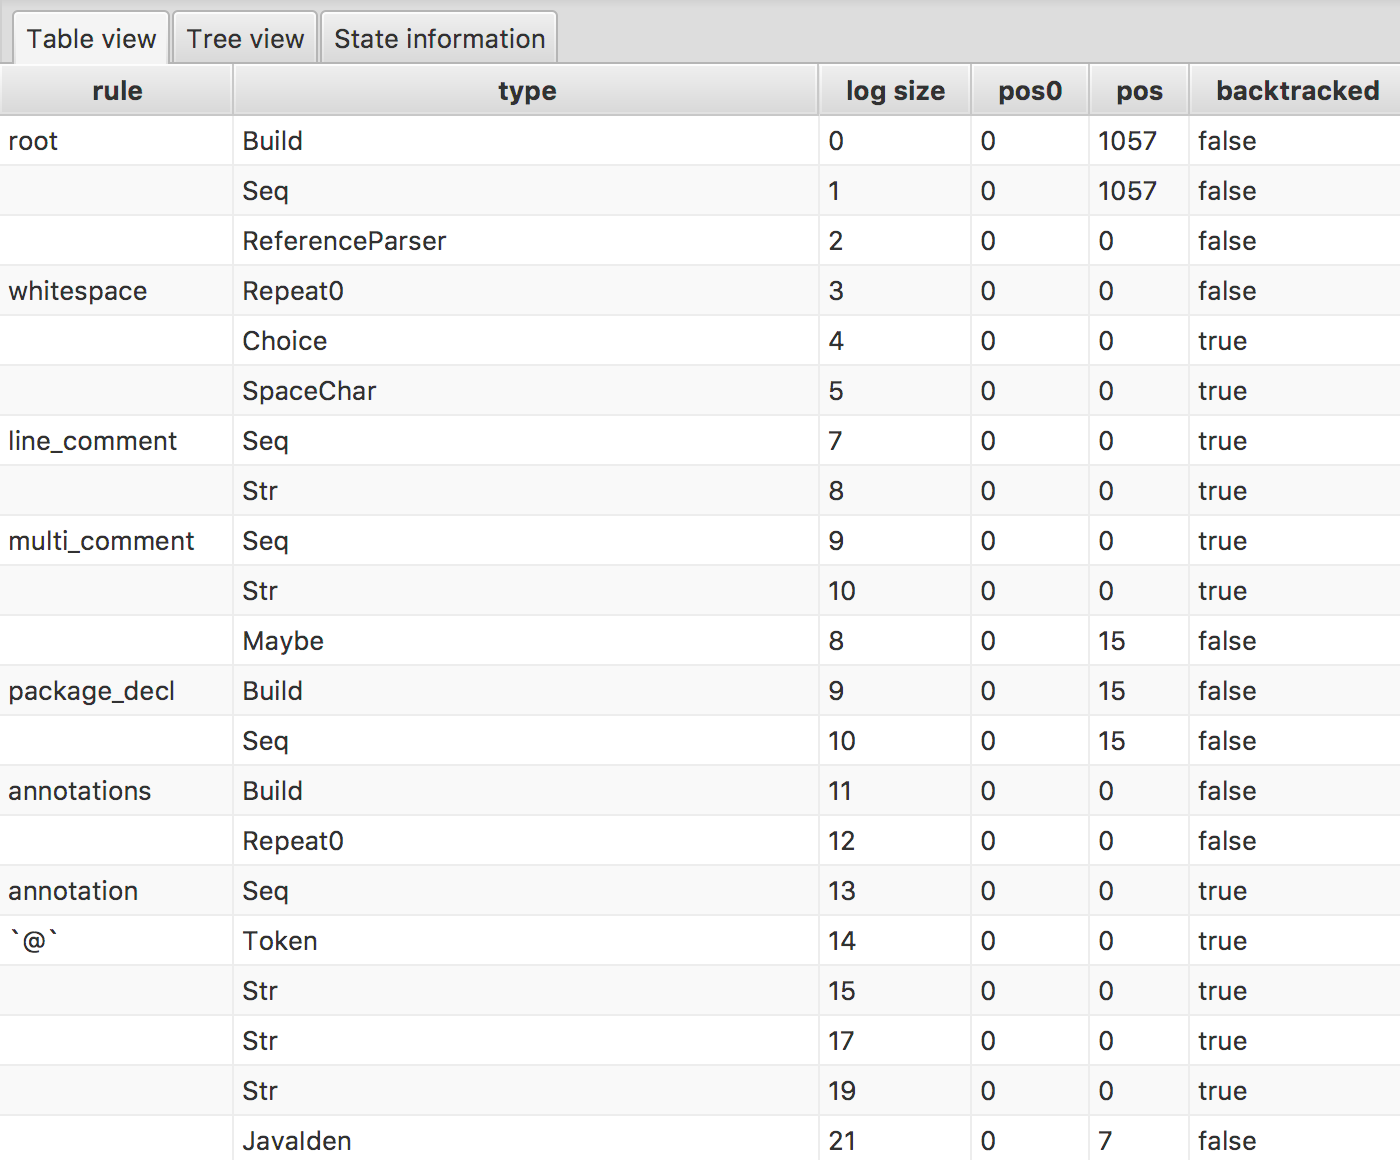
\includegraphics[width=.7\textwidth] {ressources/tableview}
			\caption{} 
			\label{fig:tableview}
		\end{figure}
		\paragraph{Tree view - Syntax tree} The tree view highlight the hierarchy of the parsers

		\begin{itemize}
			\item highlight the hierarchy between parsers and rules
		\end{itemize}

		\begin{figure}[h]
			\centering
			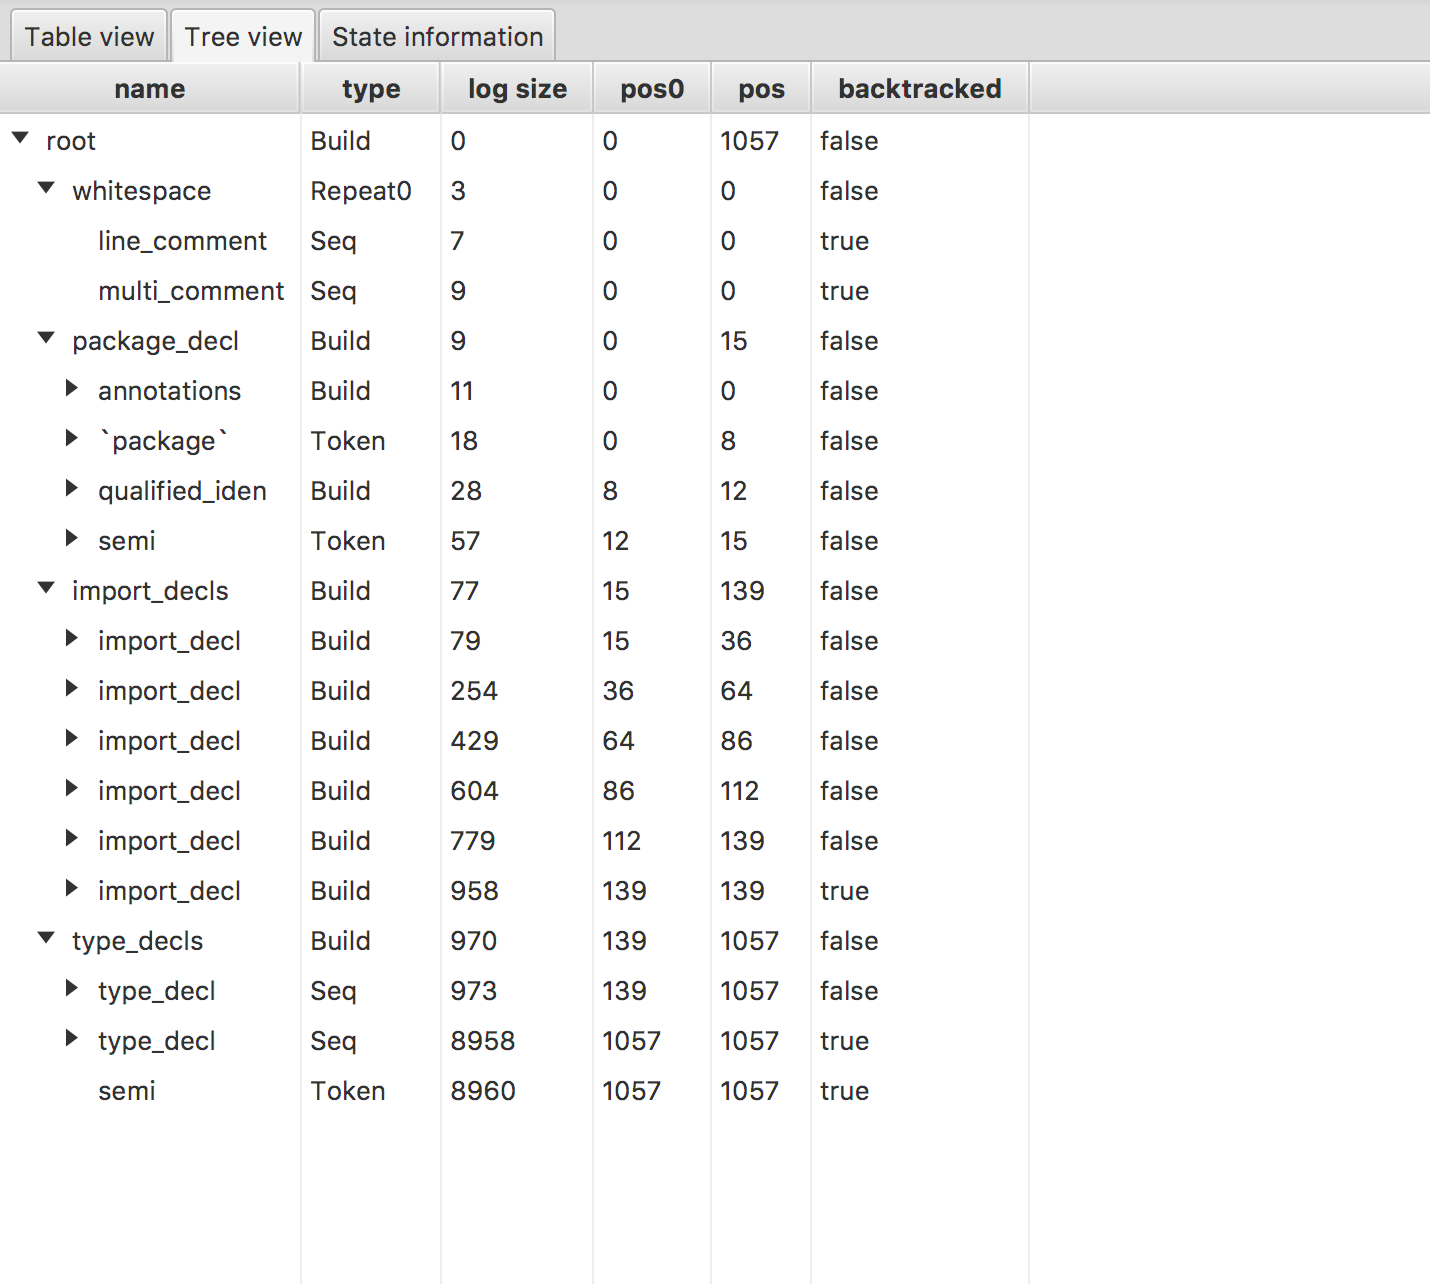
\includegraphics[width=.7\textwidth] {ressources/treeview}
			\caption{} 
			\label{fig:treeview}
		\end{figure}

		\paragraph{State information} This tab display the current state


		%%%---%%%---%%%---%%%---%%%---%%%---%%%---%%%---%%%---%%%---%%%---%%%---%%%---%%%---%%%---%%%---%%%---%%%---%%%---%%%---%%%---%%%---%%%---%%%---%%%
		\subsection{Filtering the informations}
		%%%---%%%---%%%---%%%---%%%---%%%---%%%---%%%---%%%---%%%---%%%---%%%---%%%---%%%---%%%---%%%---%%%---%%%---%%%---%%%---%%%---%%%---%%%---%%%---%%%

		\begin{itemize}
			\item all this information is overwhelming and not very usefull (like a dump of info)
			\item filter allow to select the relevant informations the user might be reasoning with
			\item filter possibilities
			\item unamed: unamed parser which doesn't match the rule one to one 
			\item backtracked
			\item no match : nodes that didn't match anything in the input but succeded
		\end{itemize}

		% Because we don't stop the execution with breakpoints, the user will get the entire execution trace and all the related information with it at once. This can be a little bit overwhelming and therefore defeat the purpose of the debugger. To facilitate the navigation of thoses information we create filtering tools. The user can decide what to display at anytime. The different filters fill in different roles. It is possible to filter the unamed parser which doesn't match the rule one to one to get a ``higher'' level view of the parsing. One can filter out the node that backtracked to see exactly how the input has been matched. Because of the nature of certain parsers, there will be nodes that didn't match anything in the input but succeded anyway and therefore didn't backtracked, those nodes are filterable as well. And finally, because the user might be interested only in the matching of a particular rule or parser, there is a search field in which we can input the name of the parser of interest to filter everything else out.

%%%---%%%---%%%---%%%---%%%---%%%---%%%---%%%---%%%---%%%---%%%---%%%---%%%---%%%---%%%---%%%---%%%---%%%---%%%---%%%---%%%---%%%---%%%---%%%---%%%
%
\chapter{Implementation}
\label{chap:impl}
%
%%%---%%%---%%%---%%%---%%%---%%%---%%%---%%%---%%%---%%%---%%%---%%%---%%%---%%%---%%%---%%%---%%%---%%%---%%%---%%%---%%%---%%%---%%%---%%%---%%%
	This chapter will present the practical implementation of the solution.

	In section \ref{sec:autumn}, we presented the overall structure of the Autumn parsing libraries. 

	The debugging logic has been implemented using hooks attached to the parsers.

%%%---%%%---%%%---%%%---%%%---%%%---%%%---%%%---%%%---%%%---%%%---%%%---%%%---%%%---%%%---%%%---%%%---%%%---%%%---%%%---%%%---%%%---%%%---%%%---%%%
\section{The debuging tool implementation}
%
%%%---%%%---%%%---%%%---%%%---%%%---%%%---%%%---%%%---%%%---%%%---%%%---%%%---%%%---%%%---%%%---%%%---%%%---%%%---%%%---%%%---%%%---%%%---%%%---%%%

%%%---%%%---%%%---%%%---%%%---%%%---%%%---%%%---%%%---%%%---%%%---%%%---%%%---%%%---%%%---%%%---%%%---%%%---%%%---%%%---%%%---%%%---%%%---%%%---%%%
	\subsection{Overview of the structure}
%
%%%---%%%---%%%---%%%---%%%---%%%---%%%---%%%---%%%---%%%---%%%---%%%---%%%---%%%---%%%---%%%---%%%---%%%---%%%---%%%---%%%---%%%---%%%---%%%---%%%

	\begin{itemize}
		\item model
		\begin{itemize}
			\item builder
			\item model compilers
			\begin{itemize}
				\item model compiler
				\item graph model compiler
			\end{itemize}
		\end{itemize}
		\item parsers interface, subparsers
		\item syntax tree STnode
	\end{itemize}

\begin{itemize}
	\item autumn
	\begin{itemize}
		\item parse state
		\begin{itemize}
			\item undoable list
			\item undoable map
		\end{itemize}
		\item grammar
	\end{itemize}
\end{itemize}

%%%---%%%---%%%---%%%---%%%---%%%---%%%---%%%---%%%---%%%---%%%---%%%---%%%---%%%---%%%---%%%---%%%---%%%---%%%---%%%---%%%---%%%---%%%---%%%---%%%
	\subsection{Hooking into the parser implementation}
%
%%%---%%%---%%%---%%%---%%%---%%%---%%%---%%%---%%%---%%%---%%%---%%%---%%%---%%%---%%%---%%%---%%%---%%%---%%%---%%%---%%%---%%%---%%%---%%%---%%%
	The debuging logic presented in the previous chapter has been implemented through the creation of a hook inside the parsers. During a debuging session, each parser invocation will instead call the debug function that will handle the debugging logic.

	\bigskip

	Originally, the parsers were implemented in a strictly functionnal fashion. Autumn defines a parser simply as a boolean function taking some input, optionally modifying the parse state, advancing the input position and finally returning a boolean indicating the success or failure of its execution. 

	\bigskip

	To implement our hook, we changed the parsers from a functional implementation to an object oriented implemention by simply wrapping the parsers function inside objects.
	A general parser interface has been created to serve as an entry point for our hook.

	\bigskip

	We called this new implementation ``naive parsers'' because we suspected that it would cause some performances issues due to constant creation of new objects during the parse, this issue was referred to as megamorphic call sites. Interestingly, after comparing the benchmark, it has been shown that the impact on the execution time wasn't significant. The results of these benchmark is discussed in chapter \ref{chap:bench}

%%%---%%%---%%%---%%%---%%%---%%%---%%%---%%%---%%%---%%%---%%%---%%%---%%%---%%%---%%%---%%%---%%%---%%%---%%%---%%%---%%%---%%%---%%%---%%%---%%%
%
	\subsection{Rewritting the grammar, the notion of model and model Compiler}
%
%%%---%%%---%%%---%%%---%%%---%%%---%%%---%%%---%%%---%%%---%%%---%%%---%%%---%%%---%%%---%%%---%%%---%%%---%%%---%%%---%%%---%%%---%%%---%%%---%%%

	The changes made to the parsers had the consequence that we had to rewrite the grammar to reflect those modifications. As discussed before, writing grammar without proper debugging tools can be a time consuming and error prone business. Moreover, to investigate the suspected performances issues related to the megamorphic call sites, we wanted to make sure that we could recreate this new grammar in such a way that we could effectively compare its performances with the previous implementation.

	\bigskip

	To do so, we created an \textbf{object graph model} representing the grammar. This model would be used to generate actual grammars using a model compiler. The first challenge was to regenerate the exact same java grammar we had before based on the model. The reason for this step was to ensure the correctness of the model, if we can regenerate the grammar from the model, then we can be sure that another grammar generate from the same model will be correct as well.

	The second compiler, baptise ``graph model compiler'' aimed to generate a java grammar based on the object oriented implementation of the parsers. It's name comes from the fact that the grammar generated is represented by a graph of connected objects. Figure \ref{fig:model-grammar} illustrate the relationship between model, model compiler and grammar.

	\bigskip

	Then, both grammar was tested on a consequential java corpus. It appeared that the performances, although slightly affected by the creation of so many objects wasn't impacted in a significant way. The results will be discussed more deeply in the chapter \ref{chap:bench}. 

	\begin{figure}[h]
		\centering
		\includegraphics[width=1\textwidth] {ressources/model-grammar}
		\caption{Chart illustrating model-grammar generation} 
		\label{fig:model-grammar}
	\end{figure}

	% \clearpage
	\bigskip

	The other motivation we had to create this framework was to simplify the writting of grammar. Autumn grammars are indeed constrained by the inlining notation of the Kotlin language that introduce a less desirable verbosity. The notation for rule definition can be greatly simplified by using this framework as one can see in the following code sample. 

	\begin{tcolorbox}
	\begin{lstlisting}
val method_ref_suffix = Build(2,
   syntax = iden,
   effect = {MaybeBoundMethodReference(it(0), it(1), 
   				it(2))}).g.d("method_ref_suffix")
	\end{lstlisting}
    \end{tcolorbox}
    \begin{tcolorbox}
	\begin{lstlisting}
val method_ref_suffix
   = iden
   .build (2, "MaybeBoundMethodReference(it(0), it(1), it(2))")

	\end{lstlisting}
    \end{tcolorbox}

	% \begin{tcolorbox}
	% \begin{verbatim}
	% val method_ref_suffix = Build(2,
 %        syntax = iden,
 %        effect = {MaybeBoundMethodReference(it(0), it(1), it(2))})
 %        		.g.d("method_ref_suffix")

 %    \end{verbatim}
 %    \end{tcolorbox}
 %    \begin{tcolorbox}
 %    \begin{verbatim}
 %    val method_ref_suffix
 %        = iden
 %        .build (2, "MaybeBoundMethodReference(it(0), it(1), it(2))")

 %    \end{verbatim}
    % \end{tcolorbox}
% 

% \begin{itemize}
% 	\item schemas qui explique la structure model/grammar.
% \end{itemize}

%%%---%%%---%%%---%%%---%%%---%%%---%%%---%%%---%%%---%%%---%%%---%%%---%%%---%%%---%%%---%%%---%%%---%%%---%%%---%%%---%%%---%%%---%%%---%%%---%%%
%
		\subsection{Syntax Tree generation}
%
%%%---%%%---%%%---%%%---%%%---%%%---%%%---%%%---%%%---%%%---%%%---%%%---%%%---%%%---%%%---%%%---%%%---%%%---%%%---%%%---%%%---%%%---%%%---%%%---%%%
	
	The AST autumn is building during the parse is abstracting some of the nodes together to reduce the size of the tree and make it more readable from a human stand-point. A consequence of this is that we don't have a direct mapping between tree nodes and grammar rules.

	\bigskip

	This is a critical part of the debuging effort. The syntax tree is build by the debuging logic, separately from autumn AST and is only build during in debugging mode.
 	For debugging purposes, backtracking nodes are kept within the tree as well. Backtracking nodes are of course marked as backtracked

 	\bigskip

	The implementation of the syntax tree is contain in the STNode class. It is the structure that holds all the informations needed to debug the grammar.

%%%---%%%---%%%---%%%---%%%---%%%---%%%---%%%---%%%---%%%---%%%---%%%---%%%---%%%---%%%---%%%---%%%---%%%---%%%---%%%---%%%---%%%---%%%---%%%---%%%

%%%---%%%---%%%---%%%---%%%---%%%---%%%---%%%---%%%---%%%---%%%---%%%---%%%---%%%---%%%---%%%---%%%---%%%---%%%---%%%---%%%---%%%---%%%---%%%---%%%
%
		\subsection{Debug logic and syntax nodes}
%
%%%---%%%---%%%---%%%---%%%---%%%---%%%---%%%---%%%---%%%---%%%---%%%---%%%---%%%---%%%---%%%---%%%---%%%---%%%---%%%---%%%---%%%---%%%---%%%---%%%

	When called the debuging logic will start building up the syntaxt tree as the different parsers get invoked. For each invoked parser, a syntax node is created graft onto the tree. The final syntax tree counts one node per parser invoked.

	One might wonder what happens when a particular parser fail and backtracked over. Nothing happens, we keep this node right inside the tree, because for debugging purposes, it can be interesting to see which node backtracked as a rule could fail to match an input while its intended purpose was to match it.

	\bigskip

	The syntax tree itself is represented by a chained structure called syntax node, or STNode. Each parser call is represented by an STNode in the tree. It holds information about the parser:

	\begin{itemize}
		\item each nodes knows information about the parser it is linked to
		\item its type
		\item if it is the definition of a rule
		\item the position in the input
		\item the size of the state log to be able to regenerate the state
		\item its parent and children
	\end{itemize}

	In the context sensitivity setting, it might be important to be able to display information related to the global parse state. The way autumn recall context is to register it within a mutable parse state. This parse state essentially works as a log whose entries represent mutations applied to this state. Each entry stores the mutation as well as a way to revert it, and later on reapply it. Therefore, it is possible by reccording the size of the log to actually regenerate the parse state corresponding to a specific parser call.

	\bigskip

	This state represent the context shared between different parsers, as such, when one parser backtracked, the mutations it applied to the parse state are reverted and removed from the log. Therefore, to be able to regenerate the parse state for backtracked parsers, we need to adapt our implementation a bit.

	\bigskip

	The debug logic is contained in the \textit{debugNode} class. Any number of additional functionality can be added by creating new hooks to the implementation of the debug function


% Usually in grammar parsing, the framework usually generate a syntax tree and let the user generate an AST derived from it. One of Autumn's specificity was that it didnt produce a Syntax tree and directly produced a AST. The problem with this approach on the debugger side is that we want to be able to see exactly which rule matched with the input and to do se we need the nodes from the tree to be in a direct mapping with the rules of the grammar.

	%%%---%%%---%%%---%%%---%%%---%%%---%%%---%%%---%%%---%%%---%%%---%%%---%%%---%%%---%%%---%%%---%%%---%%%---%%%---%%%---%%%---%%%---%%%---%%%---%%%
	\section{Plugin Implementation}
	%%%---%%%---%%%---%%%---%%%---%%%---%%%---%%%---%%%---%%%---%%%---%%%---%%%---%%%---%%%---%%%---%%%---%%%---%%%---%%%---%%%---%%%---%%%---%%%---%%%
	Intellij IDE's interace uses java SWING. Considering that the entire project has been code in Kotlin, we were reluctant to use this out of style implementation of GUI.

	\paragraph{}

 	Because we needed to our implementation to interoperate with the SWING components of the IDE, we considered javaFX \cite{oracle_javafx} which is an evolution of SWING by Oracle, but like its predecessor it's written in java and still very verbose. In the end, we were seduced by the tornadoFX \cite{tornadofx} framework, coded in kotlin, it is build on top of of javaFX, assuring seamless interoperability with SWING as well as providing the powerful syntax of Kotlin.

		%%%---%%%---%%%---%%%---%%%---%%%---%%%---%%%---%%%---%%%---%%%---%%%---%%%---%%%---%%%---%%%---%%%---%%%---%%%---%%%---%%%---%%%---%%%---%%%---%%%
		\subsubsection{TornadoFX framework - reasons why we used tornadofx}
		%%%---%%%---%%%---%%%---%%%---%%%---%%%---%%%---%%%---%%%---%%%---%%%---%%%---%%%---%%%---%%%---%%%---%%%---%%%---%%%---%%%---%%%---%%%---%%%---%%%
		Present the strenght of tornadoFX vs standard SWING. Highlight the fact that it is written in kotlin and therefore can harness the strenght of the language and at the same time, since its based on javaFX it guaranteed its interoperability with SWING and therefore blend seemlessly with the IDE.

		Present some example of how it can dramatically reduce the effort needed to build up a GUI compared to SWING.
		% User interfaces are becoming increasingly critical to the success of consumer and business applications. With the rise of consumer mobile apps and web applications, business users are increasingly holding enterprise applications to a higher standard of quality. They want rich, feature-packed user interfaces that provide immediate insight and navigate complex screens intuitively. More importantly, they want the application to adapt quickly to business changes on a frequent basis. For the developer, this means the application must not only be maintainable but also evolvable. TornadoFX seeks to assist all these objectives and greatly streamline the coding of JavaFX UI's.
		% While much of the enterprise IT world is pushing HTML5 and cloud-based applications, many businesses are still using desktop UI frameworks like JavaFX. While it does not distribute to large audiences as easily as web applications, JavaFX works well for "in-house" business applications. Its high-performance with large datasets (and the fact it is native Java) make it a practical choice for applications used behind the corporate firewall.
		% JavaFX, like many UI frameworks, can quickly become verbose and difficult to maintain. Fortunately, the release of Kotlin has created an opportunity to rethink how JavaFX applications are built.

		% In February 2016, JetBrains released Kotlin, a new JVM language that emphasizes pragmatism over convention. Kotlin works at a higher level of abstraction and provides practical language features not available in Java. One of the more important features of Kotlin is its 100% interoperability with existing Java libraries and codebases, including JavaFX.
		% While JavaFX can be used with Kotlin in the same manner as Java, some believed Kotlin had language features that could streamline and simplify JavaFX development. Well before Kotlin's beta, Eugen Kiss prototyped JavaFX "builders" with KotlinFX. In January 2016, Edvin Syse rebooted the initiative and released TornadoFX.
		% TornadoFX seeks to greatly minimize the amount of code needed to build JavaFX applications. It not only includes type-safe builders to quickly lay out controls and user interfaces, but also features dependency injection, delegated properties, control extension functions, and other practical features enabled by Kotlin. TornadoFX is a fine showcase of how Kotlin can simplify codebases, and it tackles the verbosity of UI code with elegance and simplicity. It can work in conjunction with other popular JavaFX libraries such as ControlsFX and JFXtras. It works especially well with reactive frameworks such as ReactFX as well as RxJava and friends (including RxJavaFX, RxKotlin, and RxKotlinFX).

		% Motivational example in the intro guide

		%%%---%%%---%%%---%%%---%%%---%%%---%%%---%%%---%%%---%%%---%%%---%%%---%%%---%%%---%%%---%%%---%%%---%%%---%%%---%%%---%%%---%%%---%%%---%%%---%%%
		\subsection{Event Handler \& Message passing}
		%%%---%%%---%%%---%%%---%%%---%%%---%%%---%%%---%%%---%%%---%%%---%%%---%%%---%%%---%%%---%%%---%%%---%%%---%%%---%%%---%%%---%%%---%%%---%%%---%%%
		implementation details of the GUI that are maybe not so relevant as we discussed ... I suppose Im gonna remove this section.



% \paragraph{side note}
% An interesting product that is in development is JPro, a web-based JavaFX container that uses no plugins. It can work with TornadoFX and JavaFX, but is still in closed beta at the time of writing. You can follow the project and wait for its availability here: https://jpro.io/

	%%%---%%%---%%%---%%%---%%%---%%%---%%%---%%%---%%%---%%%---%%%---%%%---%%%---%%%---%%%---%%%---%%%---%%%---%%%---%%%---%%%---%%%---%%%---%%%---%%%
	\subsection{Limitations}

	%%%---%%%---%%%---%%%---%%%---%%%---%%%---%%%---%%%---%%%---%%%---%%%---%%%---%%%---%%%---%%%---%%%---%%%---%%%---%%%---%%%---%%%---%%%---%%%---%%%

		\subsection{execution thread}
		\begin{itemize}
			\item intellij doesnt allow certain instructions to be called from another thread than the one expects.
			\item tornadoFX works in its own thread, so some functionallity are not possible as it is
		\end{itemize}
%%%---%%%---%%%---%%%---%%%---%%%---%%%---%%%---%%%---%%%---%%%---%%%---%%%---%%%---%%%---%%%---%%%---%%%---%%%---%%%---%%%---%%%---%%%---%%%---%%%
%
\chapter{validation}
\label{chap:bench}
%
%%%---%%%---%%%---%%%---%%%---%%%---%%%---%%%---%%%---%%%---%%%---%%%---%%%---%%%---%%%---%%%---%%%---%%%---%%%---%%%---%%%---%%%---%%%---%%%---%%%

\section{Benchmarking}

\subsection{Profiling excution time}

As mentionned earlier, one interesting aspect to look at in term of performances was the megamorphic call sites. To perfom a meaningful Benchmarking, a consequent java framework \cite{java_corpus} has been used as a input corpus for Autumn to parse. The framework itself contains 7800 files and more than a million lines, therefore representing a fairly big project.

\bigskip

Because of megamorphic call sites, it was expected that the new implementation of the parsers would be much slower. It indeed does have an impact on performances increasing the relative execution time by an order of magnitude of 25\%, which might be considered significant, although considering the overall execution time with respect to the size of the input (1.2 Million lines), it can be argued that this loss of performances doesnt impact the project so much.

\bigskip

Figures \ref{fig:prof_ggram} provide an illustration of the profiler for the functional parser implementation while figure \ref{fig:prof_javag} illustrate the results of the profiler for the object oriented implementation of the parsers.

		\begin{figure}[h]
			\centering
			\includegraphics[width=.8\textwidth] {ressources/prof_javag}
			\caption{Profiler for the benchmark with functional parser implementation} 
			\label{fig:prof_ggram}
		\end{figure}

		\begin{figure}[h]
			\centering
			\includegraphics[width=.8\textwidth] {ressources/prof_ggram}
			\caption{Profiler for the benchmark with object oriented implementation} 
			\label{fig:prof_javag}
		\end{figure}


\bigskip

Additionally, we also ran the benchmark for this corpus in debug mode for sake of comprehensivity. Although it is expected that our debugger will be used on smaller test inputs to verify the correctness of a portion of the grammar at a time, it is still relevant to measure the impact the overhead introduced by the debugger has on performances. As figure \ref{fig:prof_debug} demonstrate, the overhead introduced increase the execution time by an order of 10. Considering that debuggers are usually used to quickly test a solution rather than mentally check the correctness of the code, an execution time of 2 minutes is not acceptable. It is although not reasonable to think that one would use the debugger in that way for huge project like this one.


		\begin{figure}[h]
			\centering
			\includegraphics[width=.8\textwidth] {ressources/prof_debug}
			\caption{Profiler for the benchmark in debug mode} 
			\label{fig:prof_debug}
		\end{figure}



\subsection{Profiling memory consumption}

	In this section we are interested in the memory consumption overhead the debugger introduced. Generally, we expect that one would use this tool on very small examples to provide actionnabe feedback as he or she design the grammar. Therefore, the memory consumption on such small examples, which would represent the majority of the usual use-cases, isn't really critical. 

	\bigskip

	Despite this assumption, if for any reason, one would be interested in running the debugger on a large project, generating and maintaining a large amount of structures could represent an issue for memory consumption and prevent the algorithm to run altogether. To study this issue, we used JProfiler \cite{JProfiler} to analyze the memory consumption of the solution.

	\bigskip

	Figure \ref{fig:memory_ggrammar} and Figure \ref{fig:memory_debug} presents the live memory consumption after parsing the same corpus used in the previous section (Java spring framework containing 1.2 million lines).

	We can observe that the structure maintained by the debugger increase the memory consumption significantly. The syntax tree alone generate more than 300MB of data, not considering the increased memory cost in the form of extra appliedSideEffects. Of course, the is no way around an increased overhead in memory consumption. Despite those observation, one might argue that, even thought the memory consumption has been increased significantly, the cheer size of the framework used for the benchmark rule out the need for additional modification for our debugger to run on bigger projects.

		\begin{figure}[h]
			\centering
			\includegraphics[width=1\textwidth] {ressources/memory_ggrammar}
			\caption{Memory consumption without debugging} 
			\label{fig:memory_ggrammar}
		\end{figure}
		\begin{figure}[h]
			\centering
			\includegraphics[width=1\textwidth] {ressources/memory_debug}
			\caption{Memory consumption with debugging}
			\label{fig:memory_debug}
		\end{figure}



	%%%---%%%---%%%---%%%---%%%---%%%---%%%---%%%---%%%---%%%---%%%---%%%---%%%---%%%---%%%---%%%---%%%---%%%---%%%---%%%---%%%---%%%---%%%---%%%---%%%
	\section{Debugger in practice}
	\label{debugexample}
	%%%---%%%---%%%---%%%---%%%---%%%---%%%---%%%---%%%---%%%---%%%---%%%---%%%---%%%---%%%---%%%---%%%---%%%---%%%---%%%---%%%---%%%---%%%---%%%---%%%

	\subsection{Examples}

	\paragraph{case study 1 : error in grammar}

	For this example, we will show how to go about to detect an error in the grammar and how our tool helps to resolve the issue.


	\paragraph{case study 2 : error in input}

	This time, the grammar will be correct, but we will introduce a mistake in the parsed input and see how the tool helps to find out where the problem is.

	\paragraph{case study 3 : error in parser definition}

	Finally, because a user could define a custom parser to handle some custom/domain specific parse state, we will introduce a mistake in the definition of a parser and see how it can be detected.


	%%%---%%%---%%%---%%%---%%%---%%%---%%%---%%%---%%%---%%%---%%%---%%%---%%%---%%%---%%%---%%%---%%%---%%%---%%%---%%%---%%%---%%%---%%%---%%%---%%%
%
\chapter{Future work}
%
%%%---%%%---%%%---%%%---%%%---%%%---%%%---%%%---%%%---%%%---%%%---%%%---%%%---%%%---%%%---%%%---%%%---%%%---%%%---%%%---%%%---%%%---%%%---%%%---%%%

	%%%---%%%---%%%---%%%---%%%---%%%---%%%---%%%---%%%---%%%---%%%---%%%---%%%---%%%---%%%---%%%---%%%---%%%---%%%---%%%---%%%---%%%---%%%---%%%---%%%
	\section{Debugger extension}
	%%%---%%%---%%%---%%%---%%%---%%%---%%%---%%%---%%%---%%%---%%%---%%%---%%%---%%%---%%%---%%%---%%%---%%%---%%%---%%%---%%%---%%%---%%%---%%%---%%%

	\subsection{Adding hooks}
	\begin{itemize}
		\item access more informations during debug
		\item create new state structure
	\end{itemize}

	\subsection{Turning the plugin into a full fledge independent software}

	\subsection{Working in tandem with the general purpose debugger}

	%%%---%%%---%%%---%%%---%%%---%%%---%%%---%%%---%%%---%%%---%%%---%%%---%%%---%%%---%%%---%%%---%%%---%%%---%%%---%%%---%%%---%%%---%%%---%%%---%%%
	\section{Autumn related}
	%%%---%%%---%%%---%%%---%%%---%%%---%%%---%%%---%%%---%%%---%%%---%%%---%%%---%%%---%%%---%%%---%%%---%%%---%%%---%%%---%%%---%%%---%%%---%%%---%%%
		\subsection{Parser implementation}
		\begin{itemize}
			\item as discussed, parsers as been reimplemented as objects.
			\item the implementation was meant to be temporary because of the suspected performances issues
			\item since this issues are neglictable, the functions can be directly integreted in the object implementation
			\item better management of memory
		\end{itemize}

	
	%%%---%%%---%%%---%%%---%%%---%%%---%%%---%%%---%%%---%%%---%%%---%%%---%%%---%%%---%%%---%%%---%%%---%%%---%%%---%%%---%%%---%%%---%%%---%%%---%%%
	\section{GUI extentions}
	%%%---%%%---%%%---%%%---%%%---%%%---%%%---%%%---%%%---%%%---%%%---%%%---%%%---%%%---%%%---%%%---%%%---%%%---%%%---%%%---%%%---%%%---%%%---%%%---%%%
	Making use of tornadoFX powerful verboseless feature, we implemented the plugin strictly following the MVC paradigm, decoupling the functionalities from the display. We worked with easy maintainability and extendability in mind at all time. 

	\paragraph{}

	The code is divided in 3 different classes, there is the Model which stores all the data. Then there is the views that define the way data will be displayed. And finally, there is a controller, the middleman that request information to the model and dispatch them to the views. The implementation make use of an event system which help decouple the controller and the view furthermore. It is therefore very easy to create new views to hook on the masterview, or replace the masterview all together, the only thing needed is to listen to the event and display the received data in the chosen way. Symmetrically, it is as easy to create new filters, or provide new information to the views by creating new events and new methods in the controller.

	Because Autumn implements stateful parsing, the users may define custom states for his parsers. It is then his responsability to create a display for it and to feed it to the plugin views. For this purpose I added an interface for the states that define a ``getRepresentation'' method.

% In test-driven development the debugger is used as a development tool given that it provides direct access to the running system [20].

% Test Driven Development: By Example
% Beck,K.:TestDrivenDevelopment:ByExample.Addison-WesleyLongman(2002)

%%%---%%%---%%%---%%%---%%%---%%%---%%%---%%%---%%%---%%%---%%%---%%%---%%%---%%%---%%%---%%%---%%%---%%%---%%%---%%%---%%%---%%%---%%%---%%%---%%%
%
\chapter{Technical background}
%
%%%---%%%---%%%---%%%---%%%---%%%---%%%---%%%---%%%---%%%---%%%---%%%---%%%---%%%---%%%---%%%---%%%---%%%---%%%---%%%---%%%---%%%---%%%---%%%---%%%
This chapter will present the important technical aspects involved in the developpement of the solution. Feel free to skip it and come back to it
as needed. (I will reference the different section at the relevant places throughout the text) (for this chapter, Im not sure if I should
have it or directly take its section and put them in the relevant places (i.e. put the IDE plugin section in the plugin chapter))

\begin{itemize}
	\item not sure if I shouldnt just discart this entire chapter because its not really relevant and the reader can find those information himself ?
	\item anyhow, clearly the less important chapter.
\end{itemize}

% 	%%%---%%%---%%%---%%%---%%%---%%%---%%%---%%%---%%%---%%%---%%%---%%%---%%%---%%%---%%%---%%%---%%%---%%%---%%%---%%%---%%%---%%%---%%%---%%%---%%%
% 	\section{Intellij IDE}
% 	%%%---%%%---%%%---%%%---%%%---%%%---%%%---%%%---%%%---%%%---%%%---%%%---%%%---%%%---%%%---%%%---%%%---%%%---%%%---%%%---%%%---%%%---%%%---%%%---%%%
% Not sure if talking about this is super relevant, but a big chunk of the thesis is about plugin developpement for intellij, 
% therefore it might be interesting to talk about it a bit ?
		%%%---%%%---%%%---%%%---%%%---%%%---%%%---%%%---%%%---%%%---%%%---%%%---%%%---%%%---%%%---%%%---%%%---%%%---%%%---%%%---%%%---%%%---%%%---%%%---%%%
		\subsection{Plugin developpement for Intellij IDE}
		%%%---%%%---%%%---%%%---%%%---%%%---%%%---%%%---%%%---%%%---%%%---%%%---%%%---%%%---%%%---%%%---%%%---%%%---%%%---%%%---%%%---%%%---%%%---%%%---%%%
Present briefly the structure of Intellij IDE and plugin structure, limitation and difficulties ? 

	%%%---%%%---%%%---%%%---%%%---%%%---%%%---%%%---%%%---%%%---%%%---%%%---%%%---%%%---%%%---%%%---%%%---%%%---%%%---%%%---%%%---%%%---%%%---%%%---%%%
	\section{Kotlin}
	%%%---%%%---%%%---%%%---%%%---%%%---%%%---%%%---%%%---%%%---%%%---%%%---%%%---%%%---%%%---%%%---%%%---%%%---%%%---%%%---%%%---%%%---%%%---%%%---%%%
	Might not be super relevant either, but since everything is made in kotlin,	maybe its interesting to at least mention it, and quickly highlight strenght of the language VS java ?

	%%%---%%%---%%%---%%%---%%%---%%%---%%%---%%%---%%%---%%%---%%%---%%%---%%%---%%%---%%%---%%%---%%%---%%%---%%%---%%%---%%%---%%%---%%%---%%%---%%%
	\section{TornadoFX framework}
	%%%---%%%---%%%---%%%---%%%---%%%---%%%---%%%---%%%---%%%---%%%---%%%---%%%---%%%---%%%---%%%---%%%---%%%---%%%---%%%---%%%---%%%---%%%---%%%---%%%
	High level presentation of important features - how it works and difference with javafx / swing ?

%%%---%%%---%%%---%%%---%%%---%%%---%%%---%%%---%%%---%%%---%%%---%%%---%%%---%%%---%%%---%%%---%%%---%%%---%%%---%%%---%%%---%%%---%%%---%%%---%%%
\chapter{Related work}
%%%---%%%---%%%---%%%---%%%---%%%---%%%---%%%---%%%---%%%---%%%---%%%---%%%---%%%---%%%---%%%---%%%---%%%---%%%---%%%---%%%---%%%---%%%---%%%---%%%

	% 6-12 pages (7- 14)
	% Discuter differente grammaire ?
	% parler de ce qui se fait en matière de parser et interface graphique



	% https://en.wikipedia.org/wiki/Parsing_expression_grammar


%%%---%%%---%%%---%%%---%%%---%%%---%%%---%%%---%%%---%%%---%%%---%%%---%%%---%%%---%%%---%%%---%%%---%%%---%%%---%%%---%%%---%%%---%%%---%%%---%%%
\section{The Moldable Debugger: a Framework for Developing Domain-Specific Debuggers}

%%%---%%%---%%%---%%%---%%%---%%%---%%%---%%%---%%%---%%%---%%%---%%%---%%%---%%%---%%%---%%%---%%%---%%%---%%%---%%%---%%%---%%%---%%%---%%%---%%%
\section{Antlr \cite{antlr}}

% \paragraph{} A translator maps each input sentence of a language to an output sentence.

% Recognition is much easier if you break it into two similar but distinct tasks or phases. The separate phases mirror how your brain reads English text. You don’t read a sentence character by character. Instead, you perceive a sentence as a stream of words. The human brain subconsciously groups character sequences into words and looks them up in a dictionary before recognizing grammatical structure. The first translation phase is called lexical analysis and operates on the incoming character stream. The second phase is called parsing and operates on a stream of vocabulary symbols, called tokens, emanating from the lexical analyzer. ANTLR automatically generates the lexical analyzer and parser for you by analyzing the grammar you provide.

% Performing a translation often means just embedding actions (code) within the grammar. ANTLR executes an action according to its position within the grammar. In this way, you can execute different code for different phrases (sentence fragments). For example, an action within, say, an expression rule is executed only when the parser is recognizing an expression.

% Some translations should be broken down into even more phases. Often the translation requires multiple passes, and in other cases, the translation is just a heck of a lot easier to code in multiple phases. Rather than reparse the input characters for each phase, it is more convenient to construct an intermediate form to pass between phases.

% This intermediate form is usually a tree data structure, called an ab- stract syntax tree (AST), and is a highly processed, condensed version of the input. Each phase collects more information or performs more computations. A final phase, called the emitter, ultimately emits output using all the data structures and computations from previous phases.

% Figure 1.1 illustrates the basic data flow of a translator that accepts characters and emits output. The lexical analyzer, or lexer, breaks up the input stream into tokens. The parser feeds off this token stream and tries to recognize the sentence structure. The simplest translators execute actions that immediately emit output, bypassing any further phases.

% \begin{figure}
% 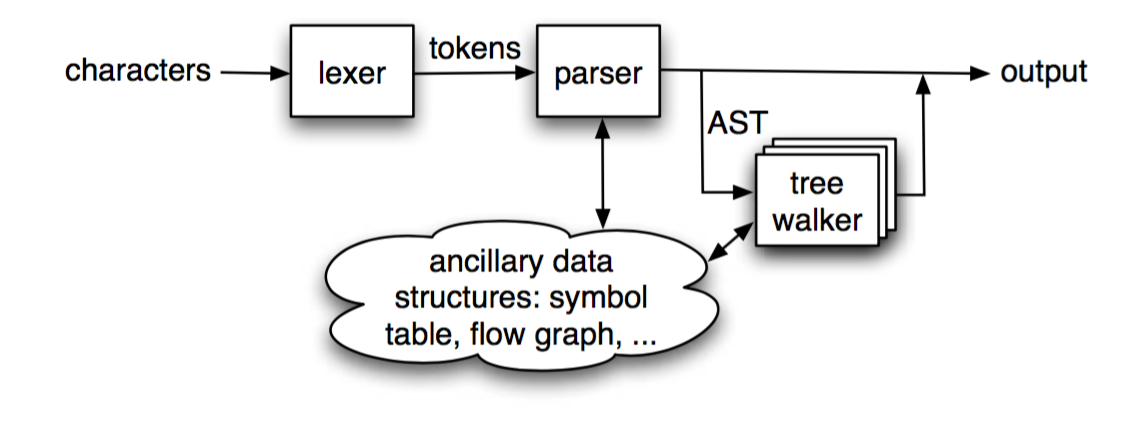
\includegraphics[width=\textwidth]{ressources/antlr1}
% \end{figure}

% \subsection{Nature of computer languages}
% Building translators with ANTLR requires you to use a formal language specification called a grammar. To understand grammars and to understand their capabilities and limitations, you need to learn about the nature of computer languages.
% The whole point of writing a grammar is so ANTLR can automatically build a program for you that recognizes sentences in that language. Unfortunately, starting the learning process with grammars and language recognition is difficult (from my own experience and from the questions I get from ANTLR users). The purpose of this chapter is to teach you first about language generation and then, at the very end, to describe language recognition. Your brain understands language generation very well, and recognition is the dual of generation. Once you understand language generation, learning about grammars and language recognition is straightforward. Here is the central question you must address concerning generation: how can you write a stream of words that transmits information beyond a simple list of items? In English, for example, how can a stream of words convey ideas about time, geometry, and why people don’t use turn signals? It all boils down to the fact that sentences are not just clever sequences of words, as Steven Pinker points out in The Lan- guage Instinct [Pin94]. The implicit structure of the sentence, not just the words and the sequence, imparts the meaning. What exactly is sen- tence structure? Unfortunately, the answer requires some background to answer properly. On the bright side, the search for a precise defini- tion unveils some important concepts, terminology, and language tech- nology along the way.

% \subsection{State machines}

% Is the lyrics state machine correct in the sense it generates valid blues sentences and only valid sentences? Unfortunately, no. The machine can also generate invalid sentences, such as “Your truck is sad and sad.” Rather than choose words (transitions) at random in each state, you could use known probabilities for how often words follow one an- other. That would help, but no matter how good your statistics were, the machine could still generate an invalid sentence. Apparently, human brains do something more sophisticated than this simple state machine approach to generate sentences. State machines generate invalid sentences for the following reasons: 

% Grammatical does not imply sensible. For example, “Dogs revert vacuum bags” is grammatically OK but doesn’t make any sense. In English, this is self-evident. In a computer program, you also know that a syntactically valid assignment such as employeeName= milesPerGallon; might make no sense. The variable types and meaning could be a problem. The meaning of a sentence is referred to as the semantics. The next two characteristics are related to syntax.

% There are dependencies between the words of a sentence. When confronted with a ], every programmer in the world has an involuntary response to look for the opening [.

% There are order requirements between the words of a sentence. You immediately see “(a[i+3)]” as invalid because you expect the ] and ) to be in a particular order (I even found it hard to type).

% So, walking the states of a state machine is too simple an approach for the generation of complex language. There are word dependencies and order requirements among the output words that it cannot satisfy. For- mally, we say that state machines can generate only the class of regular languages. As this section points out, programming languages fall into a more complicated, demanding class, the context-free languages. The difference between the regular and context-free languages is the differ- ence between a state machine and the more sophisticated machines in the next section. The essential weakness of a state machine is that it has no memory of what it generated in the past. What do we need to remember in order to generate complex language?

% To reveal the memory system necessary to generate complex language, consider how you would write a book. You don’t start by typing “the” or whatever the first word of the book is. You start with the concept of a book and then write an outline, which becomes the chapter list. Then you work on the sections within each chapter and finally start writ- ing the sentences of your paragraphs. The phrase that best describes the organization of a book is not “sequence of words.” Yes, you can read a book one word at a time, but the book is structured: chap- ters nested within the book, sections nested with the chapters, and paragraphs nested within the sections. Moreover, the substructures are ordered: chapter i must appear before chapter i+1. “Nested and ordered” screams tree structure. The components of a book are tree structured with “book” at the root, chapters at the second level, and so on.

% Interestingly, even individual sentences are tree structured. To demon- strate this, think about the way you write software. You start with a concept and then work your way down to words, albeit very quickly and unconsciously using a top-down approach. For example, how do you get your fingers to type statement x=0; into an editor? Your first thought is not to type x. You think “I need to reset x to 0” and then decide you need an assignment with x on the left and 0 on the right. You finally add the ; because you know all statements in Java end with ;. The image in Figure 2.2, on the following page, represents the implicit tree structure of the assignment statement. Such trees are called derivation trees when generating sentences and parse trees when recognizing sen- tences.

% It turns out that the humble stack is the perfect memory structure to solve both word dependency and order problems.4 Adding a stack to a state machine turns it into a pushdown machine (pushdown automa- ton). A state machine is analogous to a stream of instructions trapped within a single method, unable to make method calls. A pushdown machine, on the other hand, is free to invoke other parts of the machine and return just like a method call. The stack allows you to partition a machine into submachines. These submachines map directly to the rules in a grammar.
% Representing pushdown machines requires a different visualization called a syntax diagram, which looks like a flowchart. There is a flow- chart-like submachine per phrase (tree structure subtree). Figure 2.4, illustrates the syntax diagram for the assignment statement sentence structure. The rectangular elements generate vocabulary symbols, and the rounded elements invoke the indicated submachine. Like a method call, the pushdown machine returns from a submachine invocation upon reaching the end of that submachine.

% This section demonstrated that pushdown machines generate syntacti- cally valid sentences. In other words, each sentence that the pushdown machine generates has a valid interpretation. The next section demon- strates that, unfortunately, some valid sentences have more than one interpretation.



% The expression 3+4*5 is not ambiguous to an adult human. It means multiply 4 by 5 and add 3, yielding 23. An elementary school student doing the operations from left to right might ask, “Why is the result not 35?” Indeed, why not? Because mathematicians have decreed it so. In fact, German mathematician Leopold Kronecker went so far as to say, “God made the natural numbers; all else is the work of man.” So, the language is ambiguous, but syntax and some precedence rules make it unambiguous.

% Within a syntax diagram, an ambiguous sentence or phase is one that the diagram can generate following more than one path. For example, a syntax diagram for C can generate statement i*j; following the path for both a multiplicative expression and a variable definition (in other words, j is a pointer to type i). To learn more about the relationship of ambiguous languages to ANTLR grammars, see Section 11.5, Ambi- guities and Nondeterminisms, on page 273. For example, Section 11.5, Arithmetic Expression Grammars, on page 275 has an in-depth discus- sion of the arithmetic expression ambiguity.

% Although syntax is sometimes insufficient to interpret sentences, the informal language definition usually has some extra rules such as pre- cedence that disambiguate the sentences. Chapter 13, Semantic Predi- cates, on page 317 illustrates how to use semantic predicates to enforce these nonsyntactic rules. Semantic predicates are boolean expressions, evaluated at runtime, that guide recognition.

% \subsubsection{vocabulary symbols}
% Just as sentences consist of phrases, vocabulary symbols have struc- ture. In English, for example, a linguist sees the word destabilize as “de.stabil.ize.”7 Similarly, the real number 92.5 is two integers sepa- rated by a dot. Humans unconsciously scan sentences with these char- acters and group them into words.
% Sentences are actually sequences of characters, but your brain sees them as sequences of words as if they were complete symbols like Chi- nese characters. This happens no matter how long the words are. For example, the word for the Hawaiian state fish (Humuhumunukunukua- pua’a) is pretty long, but you read it as one symbol (pronouncing it is a lot harder). Your brain somehow implicitly forms words from the char- acters and looks them up in a dictionary of sorts.

% To mimic the technique your brain uses to recognize sentences, you need to separate the language-level processing from the vocabulary- level processing into two complete recognizers. The language-level rec- ognizer is usually called the parser, and the vocabulary recognizer is usually called the scanner, lexical analyzer, or lexer. Lexers create tokens9 (vocabulary symbols) and pass them to the parser. The only difference between the two recognizers is that the parser recognizes grammatical structure in a stream of tokens while the lexer recognizes structure in a stream of characters. Both perform essentially the same task, and ANTLR implements both using the same strategy.

% Separating the parser and lexer might seem like an unnecessary com- plication if you’re used to building recognizers by hand; however, the separation reduces what you have to worry about at each language level. You also get several implementation advantages: 

% The parser can treat arbitrarily long character sequences as sin- gle tokens. Further, the lexer can group related tokens into token “classes” or token types such as INT (integers), ID (identifiers), FLOAT (floating-point numbers), and so on. The lexer groups vocabulary symbols into types when the parser doesn’t care about the indi- vidual symbols, just the type. For example, the parser doesn’t care which integer is approaching on the input stream, just that it is an integer. Also, the parser does not have to wonder whether the next vocabulary symbol is an integer or floating-point number. The lexer can figure this out beforehand and send token type INT or FLOAT accordingly, allowing the parser to be much simpler.


% The parser sees a pipeline of tokens, which isolates it from the token source. The source of the tokens is irrelevant. For efficiency reasons, you want to save the results of lexing a character stream in a number of situations. For example, interpreters walk the same program statements multiple times during a loop. Once your lexer has tokenized the input, the parser can walk the same token buffer over and over. Some compilers (C and C++ come to mind) can even save tokenized header files to avoid repeatedly tokenizing them.

% The lexer can filter the input, sending only tokens of interest to the parser. This feature makes it easy to handle whitespace, com- ments, and other lexical structures that you want to discard. For example, if comments were passed to the parser, the parser would have to constantly check for comment tokens and filter them out. Instead, the lexer can simply throw them out, as shown in Fig- ure 2.7, on the previous page, or pass them to the parser on a hidden channel, as shown in Figure 2.8. The tokens on the hid- den channel are marked with an “x.” Note that the channel is an integer and you can put tokens on any channel you want, but the parser listens to only one channel. For more information about token channels, see Section 4.3, Lexical Rules, on page 107 and classes Token, CommonToken, and CommonTokenStream in the org.antlr.runtime package.

% At this point, you have the entire language generation picture. Sen- tences are not ingenious word sequences. Complex language generation enforces word dependencies and order requirements. Your brain enforces these constraints by subconsciously creating a tree structure. It does not generate sentences by thinking about the first word, the second word, and so on, like a simple state machine. It starts with the overall sentence concept, the root of the tree structure. From there the brain creates phrases and subphrases until it reaches the leaves of the tree structure. From a computer scientist’s point of view, generating a sentence is a matter of performing a depth-first tree walk and “saying” the words represented by the leaves. The implicit tree structure conveys the meaning.
% Sentence recognition occurs in reverse. Your eyes see a simple list of words, but your brain subconsciously conjures up the implicit tree structure used by the person who generated the sentence. Now you see why language recognition is the dual of language generation. ANTLR builds recognizers that mimic how your brain recognizes sentences. The next section gives you an intuitive feel for what sentence recog- nition by computer means. Afterward, you will be in good shape for Chapter 4, ANTLR Grammars, on page 86.

% The ANTLR parser generator accepting a larger class of grammars than LL(k) and generating recursive-descent parsers that are very similar to what a programmer would build by hand. 

\begin{itemize}
	\item ANTLR parser generator accepts a larger class of grammars than LL(k)
\end{itemize}
% \paragraph{SYNTAX DIAGRAM AND LOOKAHEAD DFA VISUALIZATION}
% 		ANTLR is a recursive-descent parser generator that accepts a large class of grammars called LL(*) that can be augmented with semantic and syntactic predicates 
% 		\subparagraph{LL($*$) and Lookahead DFA}
% 		ANTLR’s core parsing strategy is called LL(*) and is a natural extension to LL(k). LL(k) parsers make parsing decisions (i.e., distinguishing between alternative productions) using at most k symbols of lookahead. In contrast, LL(*) parsers can scan arbitrarily far ahead. Because LL(k) lookahead is bounded, the lookahead language is regular and can be encoded within an acyclic deterministic finite automaton (DFA) [6]. LL(*) simply allows cycles in the lookahead DFA. Lookahead decisions for LL(*) are no different than LL(k) decisions in that, once an alternative is predicted, LL parsing of that alternative proceeds normally.

% 		LL(*) represents a much larger class of grammars than LL(k) because parsing decisions can see past arbitrarily-long common left-prefixes. 

% 		A better solution is to recognize that, while this lookahead language is infinite, it is still regular and so there must be a (cyclic) DFA that recognizes sentences in that lookahead language. ANTLR automatically creates these lookahead DFA and makes them available to ANTLRWorks. Figure 1 is an ANTLRWorks screen shot showing a portion of the grammar as well as the lookahead DFA for the parsing decision in rule def. Being able to examine the lookahead DFA for a particular decision is very helpful when debugging grammars. Often it is not clear why a rule parses a certain input sequence improperly. Tracing that input sequence through the lookahead DFA reveals where it splits off down the wrong path, ultimately predicting the wrong alternative (currently ANTLRWorks does not visually step through the lookahead DFA).

% 		ANTLR’s use of a lookahead DFA at a decision point avoids the need for the full parser to backtrack. Running this DFA is much more efficient than running the general recursive-descent parsing process for each alternative for several reasons. First, the DFA lookahead process stops as soon as it reaches a point at which it can decide between the alternatives, and therefore it usually only looks at the first few tokens, even in a large recursive grammar rule. Second, the DFA lookahead process does not execute grammar actions, so there is no danger of executing them more than once or having to undo them.

% 		LL(*) does not approximate the distinguishing lookahead language nor the entire context-free grammar. A grammar is only LL(*) when the lookahead needed to distinguish alternative produc- tions is regular for each decision. This does not mean that the language generated by the grammar itself must be regular, however. The language generated by the following LL(1) rule is not regular, but the lookahead language used to distinguish productions is regular (’(’ or INT):

% 		\begin{verbatim}
% 	e : ’(’ e ’)’ // ’(’ predicts this alternative
% 	  | INT       // INT predicts this alternative
% 	  ;
%   		\end{verbatim}

%   		Not all lookahead languages are regular. When the lookahead computation encounters recursion reachable by more than one alternative, for example, the analysis algorithm fails rather than ap- proximating the lookahead. In this case, ANTLR can still generate a parser that uses backtracking to distinguish the alternatives at run-time. In practice, this means that ANTLR can accept any non-left-recursive grammar without complaint.


	\subsection{Antlrworks}

\begin{itemize}
	\item development environment for ANTLR grammars - parser nondeterminism visualizer (syntax diagrams and a time-traveling)
	\item grammar-aware editor with refactoring and navigation features, 
	\item a grammar interpreter
	\item domain-specific grammar debugger. 
\end{itemize}
	

	% ANTLRWorks’ primary contributions are a parser nondeterminism visualizer based upon syntax diagrams and a time-traveling debugger that pays special attention to parser decision-making by visualizing lookahead usage and speculative parsing during backtracking.

	% compute and display the parse tree associated with a particular input sequence and start rule—all without requiring a complete grammar and without having to generate code, compile, and run the application incorporating the parser.

	% It can rewind and replay the parse multiple times by re-executing the events without having to restart the actual parser. (my solution doesnt actually do time travel but provides as relevant information by being able to regenerate a state for a given parser and analyze the state of the system at the time of its execution)

	% The debugger dynamically displays a parser’s input stream, parse tree, generated abstract syntax tree (AST), rule invocation stack, and event stream as the user traces through the parser execution. The grammar, input, and tree display panes are always kept in sync so that clicking on, for example, an AST node shows the grammar element that created it and the token within the input stream from which it was created. ANTLRWorks has breakpoints and single-step facilities that allow programmers to stop the parser when it reaches a grammar location of interest or even an input phrase of interest. Sometimes it is useful to jump to a particular event (such as a syntax error) within the parse and then back up to examine the state of the parser before that event. To accommodate this, ANTLRWorks has a “step backwards” facility.

	% Complex language problems are often broken down into multiple phases with the first phase parsing the input and building an intermediate-form AST. This AST is then passed between multiple tree walkers to glean information or modify the AST. ANTLR accepts tree grammars and can automatically generate tree walkers, again in the form of a recursive-descent parser. The ANTLRworks debugger graphically illustrates the node-by-node construction of ASTs as the parser being debugged constructs these nodes. ASTs grow and shrink as the developer steps forward and backwards in the parse. ANTLR treats tree grammars just like parser grammars except that the input is a tree instead of a flat token sequence. In the ANTLRWorks debugger, programmers can set breakpoints in the input tree and single step through tree grammars to detect errors just like when debugging a token stream parser.

	
	% \subparagraph{Semantic Predicates}
	% Most programming languages are context-sensitive even though we describe them with context-free grammars for parsing efficiency reasons. Context-sensitive constructs are resolved with semantic actions during or after parsing to verify semantic validity. For example, “x=y;” only makes sense in the context of a visible variable declaration for y (and x in languages that require variables to be declared before use). In this case, context affects the validity, but not the meaning of the phrase. Syntax alone is sufficient to determine that the phrase is an assignment statement.

	% Inescapable context-sensitivity occurs when the proper interpretation of a phrase relies on in- formation about the surrounding context. Because there is no way to specify context in a pure context-free grammar, context-sensitivity results in ambiguous grammars. Ambiguous grammars can generate the same phrase in more than one way because the alternative productions cannot be predicated upon context. An ambiguous context-free grammar then has no deterministic parser (a parser that chooses exactly one phrase interpretation), rendering deterministic parsing tools based on pure context-free grammars ineffective in this case.

	% ANTLR augments context-free grammars with semantic predicates that can specify the semantic validity of applying a production, thus, providing a context-sensitive parsing mechanism. ANTLR is applicable to languages such as C++ that present a number of challenging parsing problems. One of the most difficult issues involves a syntactic ambiguity that must be resolved with symbol table information. Consider phrase C++ expression “T(34)”. This phrase can be either a constructor style typecast or a method call depending on whether T is a type name or a method name.

	% \subparagraph{Syntactic Predicates and Backtracking}
	% One weakness of the LL(*) approach is that a DFA does not have a stack and consequently cannot see past nested language structures; that is, LL(*) cannot see past recursive rule invocations to what lies beyond. To overcome this limitation, ANTLR supports syntactic predicates that predicate alter- native productions with a context-free lookahead language rather than the weaker regular lookahead language used by LL(*). Syntactic predicates not only increase the strength of LL(*) by providing a controlled backtracking mechanism, but they also provide a means of resolving grammar ambiguities.

	\paragraph{RAPID PROTOTYPING - time travel}

	
	My solution doesnt actually do time travel but provides as relevant information by being able to regenerate a state for a given parser and analyze the state of the system at the time of its execution

	% In order to develop a correct grammar quickly, the developer needs the ability to test rules as they are written. As the grammar grows, the developer adds rules to an existing base of tested rules, making it easier to track down parse errors (the errors are most likely in any newly added rules). The developer needs more than just a yes or no answer as to whether or not the input sequences match—they need parse trees, which describe exactly how the grammar matched the input sequences. Ideally, this testing would be done without code generation and target-language compilation in order to provide instantaneous feedback.

	% ANTLRWorks supports rapid grammar development by using ANTLR’s built-in interpreter, thus, providing immediate feedback during development (Meta-Environment [11] [19], TextTransformer [20], and LAUNCHPADS [21] also have interpreters).

% 	\paragraph{GRAMMAR DEBUGGER}
% 	Completing a grammar project involves verifying that the resulting parser matches input correctly, detects erroneous input, and builds a proper data structure or emits proper output. By single stepping and using breakpoints, a debugger helps clear up grammar issues but more importantly highlights which user actions are executed and in what order. Tracing through a grammar also helps track down errors in tree construction.

% 	While all of this can be accomplished clumsily using a generic programming language debugger, generic debuggers offer little more than stepping through methods and evaluating raw expressions. ANTLRWorks’ debugger, on the other hand, focuses on the higher level, domain-specific data struc- tures and processes associated with language recognition. ANTLRWorks displays input streams, parser lookahead, parse trees, parse stacks, and ASTs as they change during recognition and ensures that all visualizations stay in sync.
% 		\subparagraph{Parse Tree Visualization}
% 		\subparagraph{Debugging syntactic predicates}
% 		\subparagraph{Socket Protocol, Debug Events, and Language-Independent Debug- ging}
% 		\subparagraph{Breakpoints and Single Stepping}
% 		\subparagraph{Rewind and Stepping Backwards}
% 		When tracking down parse errors or problems related to improperly recognized input sequences, often the most crucial piece of information is what happens right before an error occurs or the parser recognizes a particular input sequence.
% 		\subparagraph{AST Visualization}

% Translators are often broken into multiple phases out of necessity because of symbol resolution issues or purely for simplicity reasons. The first phase is a parser that builds ASTs (and possibly other data structures such as a symbol table). When the grammar produces an incorrect AST, it can be difficult to track down exactly where in the grammar the erroneous subtree is created. ANTLRWorks visually displays ASTs as they are built so that the developer can single step through the grammar at the appropriate input position to discover why the improper tree is being created. The developer can view trees as two-dimensional graphs or as hierarchal lists, which are sometimes easier to visualize for very large inputs. Finally, as with the parse trees, ANTLRWorks shows the relationship between AST nodes, the input stream, and the grammar.
% 		\subparagraph{Debugging Tree Parsers}
% 		\subparagraph{related word}
% 		There are numerous tools related to grammar development environments with graphical interfaces. Most of them are academic, but there are some commercial tools. Some of the academic tools are focused on generating language development editors or other applications using generative pro- gramming from syntax and semantic specifications. ANTLRWorks is tightly focused on grammar development itself rather than grammar development as a means to creating another application. In that sense, ANTLRWorks has more in common with commercial tools, which are typically parser generators that come with grammar development environments.

% Every commercial grammar development tool has a debugger, but only ProGrammar and Text- Transformer have the data-centric breakpoint feature. ANTLRWorks has three main advantages: (1) its rewind and replay mode based on the event stream, (2) its ability to attach to a remote parser running on another machine, (3) its ability to debug parsers written in any language.

% There are a number of academic tools that allow you to develop grammars such as ASF+SDF’s Meta-Environment [11], LAUNCHPADS [21], Synthesizer Generator [30] (has now become com- mercial), SmartTools [31], LISA [32], and GTB [33] (Grammar ToolBox). Meta-Environment has grammar-aware editing, on-the-fly parser generation (supporting immediate grammar testing), GLR parse forest visualization, and some nice features that identify grammar issues such as useless sym- bols, typos, and inconsistent priorities and associativity. Meta-Environment can also generate syntax highlighters and debuggers for languages described by grammars, which includes debugging its own grammars [19]. ANTLRWorks’ debugger is less general because it works only on ANTLR grammars but is commensurately simpler and more task specific.


% LISA has a number of features that are similar to ANTLRWorks including a grammar-aware editor, BNF viewer, syntax tree viewer, and automata visualizer. Like Meta-Environment and Syn- thesizer Generator, LISA can automatically generate syntax directed editors and other visualization tools.
% While GTB has a variety of visualization views to show grammars, finite automata, and grammar dependency graphs, GTB is not strictly speaking an interactive grammar development environment. In the related world of natural language processing, Allman and Beale [34] provide a system for building natural language grammars using a visual interface and also contains a grammar debugger. DDF [35] (DSL Debugger Framework) is a set of Eclipse plugins for debugging domain specific languages described with ANTLR grammars. Aspects are used to weave in support code that maps the generated general purpose code back into the domain specific language source code. DDF reuses the existing Java Eclipse general debugger to debug domain specific languages. DDF is similar to ANTLR Studio in that both map generated code back to a domain specific language, (an ANTLR grammar in ANTLR Studio’s case and the domain specific language source code in DDF’s case). In
% contrast, ANTLRWorks uses a custom parser debugger that works with any target language. Finally, we understand that a grammar development environment for SableCC [36] is under
% construction.


%%%---%%%---%%%---%%%---%%%---%%%---%%%---%%%---%%%---%%%---%%%---%%%---%%%---%%%---%%%---%%%---%%%---%%%---%%%---%%%---%%%---%%%---%%%---%%%---%%%
\section{Ohm}
%%%---%%%---%%%---%%%---%%%---%%%---%%%---%%%---%%%---%%%---%%%---%%%---%%%---%%%---%%%---%%%---%%%---%%%---%%%---%%%---%%%---%%%---%%%---%%%---%%%


\appendix

% \chapter{Additional}
% Lorem ipsum dolor sit amet, consectetur adipiscing elit, sed do eiusmod tempor incididunt ut labore et dolore magna aliqua. Ut enim ad minim veniam, quis nostrud exercitation ullamco laboris nisi ut aliquip ex ea commodo consequat. Duis aute irure dolor in reprehenderit in voluptate velit esse cillum dolore eu fugiat nulla pariatur. Excepteur sint occaecat cupidatat non proident, sunt in culpa qui officia deserunt mollit anim id est laborum.


\begin{thebibliography}{9}

\bibitem{intellijdoc} The jetbrains intelliji platform documentation, 
	\url{http://www.jetbrains.org/intellij/sdk/docs/basics/architectural_overview/file_view_providers.html}, June 2017.

\bibitem{ohmdoc} Ohm, a parser generator consisting of a library and a domain-specific language.
	\url{https://github.com/harc/ohm}, 2017.	

\bibitem{moldable} The Moldable Debugger: A Framework for Developing Domain-Specific Debuggers
	\url{https://link.springer.com/chapter/10.1007/978-3-319-11245-9_6}.

\bibitem{graphpars}A graph grammar approach to graphical parsing
	\url{http://ieeexplore.ieee.org/document/520809/}.

\bibitem{autumn1} 
Laurent Nicolas and Mens Kim.
Parsing Expression Grammars Made Practical.
SLE, 2015.

\bibitem{autumn2} 
Laurent Nicolas and Mens Kim.
Taming Context-Sensitive Languages with Principled Stateful Parsing.
SLE, 2016.	

\bibitem{} 
David R. Hanson and Jeffrey L. Korn. :
A Simple and Extensible Graphical Debugger.
Proceedings of the USENIX Annual Technical Conference, January 6-10, 1997. 173–184
% \url{https://www.usenix.org/legacy/publications/library/proceedings/ana97/full_papers/hanson/hanson.html}

\bibitem{}
petit parser
28. Renggli, L., Ducasse, S., Gˆırba, T., Nierstrasz, O.: Practical dynamic grammars
for dynamic languages. In: Proc. DYLA. (2010)

\bibitem{} TornadoFX
	\url{https://edvin.gitbooks.io/tornadofx-guide/content/4.%20Basic%20Controls.html}

\bibitem{} psi cookbook
	\url{http://www.jetbrains.org/intellij/sdk/docs/basics/psi_cookbook.html}

\bibitem{oracle_javafx} Oracle, javaFX
	\url{http://docs.oracle.com/javase/8/javase-clienttechnologies.htm}

\bibitem{tornadofx} TornadoFX guide
	\url{https://edvin.gitbooks.io/tornadofx-guide/content/1.%20Why%20TornadoFX.html}

\bibitem{antlr} Terence J. Parr. The Definitive ANTLR Reference: Building Domain-Specific Languages. 
	The Pragmatic Programmers, 2007. ISBN 0-9787392-5-6.

\bibitem{} \texttt{Terence Parr, Jean Bovet.} ANTLRWorks: An ANTLR Grammar Development Environment, UNPUBLISHED DRAFT.

\bibitem{PEG} \texttt{Bryan Ford.} Parsing Expression Grammars: A Recognition-based Syntactic Foundation. In POPL, pages 111–122. ACM, 2004.

\bibitem{CFG} \texttt{Theodore Norvell.} A Short Introduction to Regular Expressions and Context Free Grammars. Software Engineering 7893, Typseset November 8, 2002
	\url{http://www.engr.mun.ca/~theo/Courses/fm/pub/context-free.pdf}

\bibitem{}DeLine, R., Bragdon, A., Rowan, K., Jacobsen, J., Reiss, S.P.: Debugger canvas: industrial experience with the code bubbles paradigm. In: ICSE. (2012) 1064–1073.

\bibitem{java_corpus} The Spring Framework, a comprehensive programming and configuration model for modern Java-based enterprise applications.
\url{https://github.com/spring-projects/spring-framework}

\bibitem{JProfiler} EJTechnology, JProfiler. Java JVM all in one profiler
	\url{http://www.ej-technologies.com/products/jprofiler/overview.html?gclid=EAIaIQobChMImda0lYLD1QIVjxbTCh1qxAXMEAAYASAAEgKca_D_BwE}

\bibitem{economicdebug} The Economic Impacts of Inadequate Infrastructure for Software Testing
\end{thebibliography}


 
% \bibitem{einstein} 
% Albert Einstein. 
% \textit{Zur Elektrodynamik bewegter K{\"o}rper}. (German) 
% [\textit{On the electrodynamics of moving bodies}]. 
% Annalen der Physik, 322(10):891–921, 1905.
 
% \bibitem{knuthwebsite} 
% Knuth: Computers and Typesetting,
% \\\texttt{http://www-cs-faculty.stanford.edu/\~{}uno/abcde.html}
% \end{thebibliography}


\end{document}

